\chapter{V\'eges Automat\'ak}

\section{DFA}

\defi Véges automata: $M=(Q,\Sigma,\delta,q_0,F)$ véges automatának $Q$ az állapotainak halmaza (véges sok), $\Sigma$ ábécé felett van értelmezve, $\delta$ az átmeneti függvénye (azaz adott betűt olvasva egy állapotban milyen új állapotba kerülünk), $q_0$ a kezdőállapota, $F$ a végállapotainak halmaza. Azon szavak halmazát, melyeket elolvasva az automata valamelyik végállapotába kerül, $L(M)$-lel jelöljük. Azt is mondjuk, hogy $M$ felismeri az $L(M)$ nyelvet \'es elfogadja az $L(M)$-beli szavakat.
R\'eszletesebben l\'asd: \url{http://en.wikipedia.org/wiki/Deterministic_finite-state_machine}. 

\begin{Exercise}[counter={sorszam}, difficulty=0]
	Legyen $Q=\{q_0,q_1\}$, $F=\{q_1\}$ és $\delta(q_i,a)=q_i$ és $\delta(q_i,b)=q_{1-i}$. Milyen nyelvet ismer fel ez az automata?
\end{Exercise}
\begin{Answer}
	Amikben p\'aratlan sok $a$ bet\H u van.
\end{Answer}

\begin{Exercise}[counter={sorszam}, difficulty=0]
	Adjunk véges automatát, mely az alábbi nyelveket ismeri fel!\\
a) $L=$ a $baba$-t tartalmazó szavak.\\
b) $L=$ az $abba$-t nem tartalmazó szavak.\\
c) $L=$ azon szavak, melyek utolsó előtti betűje $b$.\\
d) $L=$ azon szavak, melyekben bármely egymásutáni öt karakterből legalább kettő $a$.\\
e) $L=$ magyar (.hu v\'eg\H u) email c\'imek.
\end{Exercise}


\begin{Exercise}[counter={sorszam}, difficulty=0]
	 Tal\'alj ki egy nyelvet, amir\H ol tudod, hogy regul\'aris-e, de a padt\'arsad nem!
\end{Exercise}


\begin{Exercise}[counter={sorszam}, difficulty=0]
	 Mutasd meg, hogy van olyan nyelv, amit semely véges automata sem tud felismerni! (Ezeket {\em nem reguláris} nyelveknek hívjuk.)
\end{Exercise}	 
\begin{Answer}
	I. Nyelvb\H ol kontinuum sok van, automat\'ab\'ol viszont csak megsz\'aml\'alhat\'o sok.\\
	II. Az $a^{n^2}$ egy konkr\'et nyelv, amir\H ol k\"onnyen bel\'athat\'o, hogy nincs hozz\'a automata, hiszen $a$-kat olvasva ciklusba esne, \'igy van egy olyan $c$, hogy ha $a^{n^2}$-et elfogadja, akkor $a^{n^2+c}$-t is.
\end{Answer}


\begin{Exercise}[counter={sorszam}, difficulty=0]
	 Adott két automata, melyek az $L_1$ ill. $L_2$ nyelveket ismerik fel. Adj automatát, amely felismeri az\\
a) $\bar L_1$ (azaz $L_1$ komplementer) nyelvet,\\
b) $L_1 \cup L_2$ nyelvet,\\
c) $L_1 \cap L_2$ nyelvet,\\
d)\hard $L_1L_2$ nyelvet. (Azaz olyan szavak, melyek felbonthatók egy $L_1$ és egy $L_2$-belire.)
\end{Exercise}
\begin{Answer}
	a) Cser\'elj\"uk meg az elfogad\'o \'es az elutas\'it\'o \'allapotokat.\\
	b-c) Vegy\"uk a k\'et automata \'allapotter\'enek szorzat\'at ($Q_1\times Q_2$) \'es azon defini\'aljuk, hogy hogyan kell tov\'abbl\'epni.\\
	d)~\hard Itt $Q_1\times P(Q_2)$ lesz az \'uj \'allapott\'er, ahol $P$ a hatv\'anyhalmazt jel\"oli.
\end{Answer}


\begin{Exercise}[counter={sorszam}, difficulty=1]
	A kétirányú véges automata abban különbözik a hagyományostól, hogy nem kötelező mindig a következ\H o bet\H ut kérnie, hanem visszamehet az előzőhöz is. (Ez bele van kódolva $\delta$-ba, hogy mikor merre lép.) Mutasd meg, hogy bármely ilyen automatához létezik egy egyirányú, amely pont ugyanazt a nyelvet ismeri fel!
\end{Exercise}	
\begin{Answer}
	Minden jobbra l\'ep\'esn\'el jegyezz\"uk fel, hogy ha az eredeti automata balra \'atl\'epne, akkor milyen \'allapotban t\'erne vissza.
	Egy ilyenb\H ol mindig ki tudjuk sz\'amolni a k\"ovetkez\H o ilyet; ut\'ana a r\'egit t\"or\"olhetj\"uk, hogy a mem\'oria konstans maradjon.
\end{Answer}	

\begin{Exercise}[counter={sorszam}, difficulty=2]
	 Azt mondjuk, hogy $x$ r\'eszsorozata $y$-nak, ha $x$-et megkaphatjuk $y$-b\'ol n\'eh\'any karakter kit\"orl\'es\'evel. Adott $L$ nyelv eset\'en jel\"olje $SUBSEQ(L)$ azon szavak halmaz\'at, amik valamely $L$-beli sz\'o r\'eszsorozatai. Mutasd meg, hogy tetsz\H oleges $L$ eset\'en $SUBSEQ(L)$ felismerhet\H o v\'eges automat\'aval, ha\\
a) a $\Sigma$ ábécé k\'etelem\H u,\\
b) b\'armely v\'eges $\Sigma$ ábécé eset\'en.
\end{Exercise}
\begin{Answer}
	Ez a Higman lemma: \url{https://en.wikipedia.org/wiki/Higman%27s_lemma}.
	A l\'enyeg, hogy a Dickson lemma er\H osebb verzi\'oja igaz: ha valami v\'egesen gener\'alt, akkor bel\H ole v\'eges sok is v\'egesen gener\'alt. Ezt lehet bizonz\'itani indukci\'oval \'es v\'egtelenes Ramsey-vel. Ezutan indukci\'oval bizony\'itjuk az \'all\'it\'ast. Kett\H ore vesz\"unk valamit, ami nincs benne, ezt kieg\'esz\'itj\"uk altern\'al\'ova, enn\'el t\"obb altern\'al\'as nem lehet, $\Z$-re Dickson. H\'aromra 123123..-ra eg\'esz\'itj\"uk ki. Egy sz\'ora vessz\"uk, am\'ig csak 1,2 v\'altakozik, azt\'an 2,3 v\'altakoz\'ast, 3,1-et stb., ilyenekb\H ol nem lehet t\"obb, mint 123-as sz\'o hossza, megint lehet Dicksonozni.
		
	Egy m\'asik neh\'ez feladat: \url{http://en.wikipedia.org/wiki/Star_height_problem}.	
\end{Answer}
%


\begin{Exercise}[counter={sorszam}, difficulty=0]
	Bemenet tizes sz\'amrendszerbeli sz\'am. Jegyeit v\'altakoz\'o el\H ojellel adjuk \"ossze, majd ezt ism\'etelgess\"uk, am\'ig egyjegy\H u sz\'amot nem kapunk. Mutassuk meg, hogy azon sz\'amok nyelve, amikre null\'at kapunk, regul\'aris.\\
b)~\veryhard Mi a helyzet, ha csak minden m\'asodikat \"osszeadunk (a t\"obbit meg elfelejtj\"uk) \'es ezt ism\'etelgetj\"uk?
\end{Exercise}
\begin{Answer}
	a) Ez pont a 11-es marad\'ek lesz, amit k\"onny\H u kisz\'amolni.
	Forr\'as: Sz\"ogi Evelin feladata.\\
	b) Bocsi, de \'en sem tudom...
\end{Answer}

\begin{Exercise}[counter={sorszam}, difficulty=0]
	Pumpálós lemma: $\forall L \textit{ reguláris } \exists n \textit{ } \forall z\in L, |z|\geq n \textit{ }\exists u,v\ne \emptyset,w:\textit{ } z=uvw \textit{ és } |uv|\leq n \textit{ és } \forall i\textit{ } uv^iw\in L$.
\end{Exercise}
\begin{Answer}
	Ez a pump\'al\'os lemma: \url{https://en.wikipedia.org/wiki/Pumping_lemma_for_regular_languages}.
	L\'enyeg, hogy v\'eges sok \'allapot miatt el\H obb-ut\'obb ugyanabba l\'ep \'ujra a g\'ep.
\end{Answer}

\begin{Exercise}[counter={sorszam}, difficulty=0]
	Döntsük el, hogy az alábbi nyelvek regulárisak-e!\\
a) prímszámok egyes számrendszerben.\\
b) négyzetszámok egyes számrendszerben.\\ 
c) négyzetszámok kettes számrendszerben.\\
d)~\hard prímszámok kettes számrendszerben.
\end{Exercise}
\begin{Answer}
	a-b) Trivi pump\'al\'os lemm\'ab\'ol. Un\'aris regul\'aris nyelvek karakteriz\'aci\'oja is egyszer\H u.\\
	c) $2^{2n}$ \'es $(2^n+1)^2$ k\"oz\'e bepump\'alhatunk.\\
	d) I. Pump\'al\'as $x$-et $ax+b$-be viszi (ahol $a=2^k$).
	Vegy\"uk ennek a transzform\'aci\'onak az orbitjait mod $p$.
	Ha kezdetben $p$ osztja $x$-et, akkor $p!$ l\'epes ut\'an is osztani fogja (ha $p\ne 2$).\\
	II. Az \'atmeneti m\'atrix miatt valamely polinomokra az $n$ hossz\'u szavak sz\'ama $p_1(n)\lambda_1^n+\ldots+p_k(n)\lambda_k^n$, ez nem lehet $2^n/n$.\\
	III. (Borda Bence) Bauer Mih\'aly t\'etel (Dirichlet speci\'alis esete) szerint v\'egtelen sok $p=k2^n+1$ alak\'u pr\'im van. Pump\'al\'as ut\'an $k2^{n+id}+1$, ami $i=p-1$-re oszthat\'o $p$-vel kis-Fermat miatt.
	
	Egy hasonl\'o feladat: \url{http://cstheory.stackexchange.com/questions/2083/proving-the-set-of-powers-of-2-over-ternary-alphabet-to-be-non-regular/2086#2086}.
\end{Answer}


\begin{Exercise}[counter={sorszam}, difficulty=0]
	a) Van-e olyan $S\subset \N$, ami kettes számrendszerben reguláris, de egyesben nem?\\
	b) És fordítva?\\
	c)~\veryhard És olyan, ami kettesben és hármasban is reguláris, de egyesben nem?
\end{Exercise}	
\begin{Answer}
	a) Van, pl.\ $2^n$.\\
	b) Nincs.\\
	c) Nem tudok egyszer\H u bizony\'it\'ast, kij\"on a Cobham T\'etelb\H ol: Let $S$ be a set of non-negative integers and let $m$ and $n$ be multiplicatively independent positive integers. Then $S$ is recognizable by finite automata in both $m$-ary and $n$-ary notation if and only if it is ultimately periodic.
	\url{https://arxiv.org/abs/1801.06704}.
	%ezt nem ertem, csak ezt: http://www.emis.ams.org/journals/BBMS/Bulletin/bul942/BRU.PDF
\end{Answer}


\section{NFA}

\defi Nemdeterminisztikus véges automata: Ugyanaz, mint a determinisztikus, csak egy állapotból többfelé is léphet. (A gráfjában egy csúcsból több azonos indexű él is kiléphet.) Akkor fogad el egy szót, ha van legalább egy olyan futása, ami elfogadja.

\begin{Exercise}[counter={sorszam}, difficulty=0]
	Mutasd meg, hogy a nemdeterminisztikus v\'eges automaták is csak reguláris nyelveket ismernek fel, azaz minden nemdeterminisztikus véges automatához van egy determinisztikus, ami ugyanazt a nyelvet fogadja el!
\end{Exercise}	
\begin{Answer}
	\'Ugy csin\'alunk nemdeterminisztikus $N$ automat\'ab\'ol egy determinisztikus $M$ automat\'at, hogy az $M$ minden \'allapota az $N$ lehets\'eges \'allapotainak egy r\'eszhalmaza. Az $a$ c\'imk\'ej\H u \'el a $(q_1,..,q_k)$-b\'ol
	a $\{q\mid \exists i q_i \stackrel a\to q\}$-ba megy.
	Azok a $(q_1,..,q_k)$ \'allapotok elfogad\'ok, amikben van $N$-beli elfogad\'o \'allapot, a $START$ pedig a $(q_{START})$ \'allapot.
\end{Answer}

\begin{Exercise}[counter={sorszam}, difficulty=0]
	Adott $L$ nyelvre $L^*$ azon szavak nyelve, amik előállnak néhány $L$-beli szó konkatenációjaként. Mutasd meg, hogy ha $L$ reguláris, akkor $L^*$ is!
\end{Exercise}	
\begin{Answer}
	Nemdeterminisztikus automat\'aval k\"onny\H u, mert meg tudjuk tippelni, hogy hol \'ernek v\'eget az $L$-beli szavak.
	Ha adott $L$-et elfogad\'o determinisztikus $M$ automata, akkor csin\'alunk bel\H ole egy $L^*$-ot felismer\H o nemdeterminisztikus $N$ automat\'at. Az $N$ \'allapotai ugyanazok lesznek, csak lesz benne p\'ar plusz \'el: az \"osszes $M$-beli elfogad\'o\'allapotb\'ol vezessen \'el pontosan ugyanazokba a cs\'ucsokba is, mint a $START$ \'allapotb\'ol.
\end{Answer}


\begin{Exercise}[counter={sorszam}, difficulty=1]
	 Az altern\'al\'o v\'eges automata egy nemdeterminisztikus v\'eges automata, melynek minden állapotához hozzá van rendelve {\bf A} vagy {\bf B}. Ez két játékos, akik előre látják az inputot, az {\bf A} jelű állapotoknál {\bf A}, a {\bf B} jelű állapotoknál {\bf B} dönt, hogy melyik állapotba lépjen tovább az automata. {\bf A} célja, hogy az automata elfogadó állapotba érjen a szó végén, míg {\bf B} célja, hogy ne. Akkor fogad el egy szót az automata, ha {\bf A}-nak van rá nyerő stratégiája, az elfogadott szavak nyelvét pedig ``felismeri'' az automata. Mutasd meg, hogy az altern\'al\'o v\'eges automaták is csak reguláris nyelveket ismernek fel!
\end{Exercise}	 
\begin{Answer}
	Lehets\'eges \'allapotok halmaz\'an csin\'aljunk egy nemdeterminisztikus automat\'at. Ha {\bf B} j\"on, akkor \"osszes lehets\'eges m\'odon l\'ep\"unk, ha {\bf A} j\"on, akkor pedig helyesen tippelve a ``j\'o ir\'anyba'' (ha van ilyen).
\end{Answer}


\begin{Exercise}[counter={sorszam}, difficulty=0] Randomizált véges automata: Ugyanaz, mint a nemdeterminisztikus, csak minden éléhez hozz\'a van rendelve egy valószínűség, ez határozza meg, hogy merre mekkora eséllyel lép. Akkor fogad el egy szót, ha a futásainak $\ge\frac{2}{3}$-a elfogadja és akkor utasítja el, ha a futásainak $\le\frac{1}{3}$-a fogadja el. Akkor ismer fel egy nyelvet, ha a nyelvbeli szavakat mind elfogadja és a nem nyelvbeli szavakat mind elutasítja (tehát semelyik szóra sem lehet határozatlan).\\
a)~\hard Mutasd meg, hogy van olyan kétirányú randomizált véges automata, ami felismeri az $L=\{a^nb^n\}$ nyelvet!\\
b)~\veryhard Mutasd meg, hogy egyirányú randomizált véges automata csak reguláris nyelveket tud felismerni!
\end{Exercise}
\begin{Answer}
	a) K\"oz\'epr\H ol bolyongjunk \'es sz\'amoljuk, hogy mikor melyik v\'eg\'ere \'er\"unk.\\
	b) Legyen $x\sim y$, ha minden $z$-re $xz\in L \Leftrightarrow yz\in L$. Ha v\'egtelen sok ilyen oszt\'aly lenne, akkor lenne egy $x,y$ p\'ar, ami k\"ozel van abban az \'ertelemben, hogy minden \'allapotban kb.\ ugyanakkora es\'ellyel van a randomiz\'alt automata miut\'an elolvasta \H oket. De ekkor minden $z$-re is kb.\ ugyanakkor\'ak lesznek az es\'elyek.
\end{Answer}









\chapter{Turing-g\'epek}

\section{Alapok}

\begin{Exercise}[counter={sorszam}, difficulty=0] 
	Készíts olyan Turing-gépet, ami a bemenetként kapott $x_1x_2\ldots x_m$ sorozatot\\
a) megkétszerezi ($x_1x_2\ldots x_m x_1x_2\ldots x_m)$.\\
b) megford\'itja ($x_mx_{m-1}\ldots x_1$),\\
c) bet\H unként megkétszerezi ($x_1x_1x_2x_2\ldots x_m x_m)$.
\end{Exercise}	 


\begin{Exercise}[counter={sorszam}, difficulty=0]
	 Konstruáljunk olyan Turing-gépet, ami\\
a) az $n$ hosszú, csupa 1-esb\H ol álló bemenetre $n$ kettes számrendszerbeli alakját adja vissza,\\
%\phantom{a)} (különben pedig azt, hogy ``{\it hibás bemenet}\,'')\\
b) ha a bemenet az $n$ szám bináris alakja, akkor $n$ darab 1-est ír ki (különben azt, hogy ``{\it hibás bemenet}\,'').
\end{Exercise}	 

%hubainal volt, de sztem tul konnyu
%\pro Az el?z? feladatot úgy is oldjuk meg, hogy ha a gép nem azt adja vissza, hogy ``{\it hibás bemenet}\,'', akkor csak $O(n)$ lépést tegyen.

\begin{Exercise}[counter={sorszam}, difficulty=0]
	 Tegyük fel, hogy van két Turing-gépünk, melyek az $f$ illetve $g$ függvényt számolják ki. Konstruáljunk olyan Turing-gépet, mely az $f\circ g$ függvényt számolja ki.
\end{Exercise}	 


\begin{Exercise}[counter={sorszam}, difficulty=0]	
a)~Konstruáljunk olyan Turing-gépet, mely az $a^nb^n$ alak\'u
szavakra $O(n)$ l\'ep\'esben ki\'irja, hogy ``{\it igen}'',
m\'as szavakra v\'egtelen sok\'aig fut.\\
b)~~Konstruáljunk olyan egyszalagos Turing-gépet, mely az $a^nb^n$ alak\'u
szavakra $O(n \log n)$ l\'ep\'esben ki\'irja, hogy ``{\it igen}'',
m\'as szavakra v\'egtelen sok\'aig fut.\\
c)~\hard Mutassuk meg, hogy ez egyszalagos gépen $o(n\log n)$ l\'ep\'esben nem lehets\'eges.
\end{Exercise}	 
\begin{Answer}
	a) Lem\'asoljuk egy m\'asik szalagra az inputot \'es ellenkez\H o ir\'anyb\'ol megy\"unk v\'egig rajtuk.\\
	b) V\'egigmegy\"unk rajta \'es minden m\'asodik karaktert kit\"or\"olve ritk\'itjuk $\log n$-szer. Ha b\'armikor elt\'er a parit\'asa az $a$-knak \'es a $b$-knek, akkor nem egyenl\H oek, k\"ul\"onben meg igen.
	(Hasonl\'oan $n$-et \'at is konvert\'alhatjuk un\'arisb\'ol bin\'arisba $\log n$ l\'ep\'esben.)\\
	c) 3.3-as tetelt itt: \url{https://doi.org/10.1016/0304-3975(85)90165-3}.
\end{Answer}

\begin{Exercise}[counter={sorszam}, difficulty=1]
	Mutassuk meg, hogy egy $k$ szalagos Turing-gép szimulálható egy 2 szalagossal úgy, hogyha az eredeti $n$ lépést tett egy adott inputra, akkor a kétszalagos legfeljebb $O(n \mathrm{\;log\,} n)$-et tegyen.
\end{Exercise}	 
\begin{Answer}
	Hennie-Stearns: Two-Tape Simulation of Multitape Turing Machines.
\end{Answer}


\begin{Exercise}[counter={sorszam}, difficulty=0]
	 Adj meg egy Turing-gépet, ami b\'armely $x$ bemenetre pontosan $2^{|x|}$ lépést tesz meg.
\end{Exercise}	 
\begin{Answer}
	A legegyszer\H ubb megold\'as tal\'an egy olvas\'o + 4 m\'asik szalagos Turing-g\'ep, aminek 4 munkaszalagja un\'aris, p\'aratlan f\'azisban $a_1+a_2$-t \'irja $b_1$-re \'es $b_2$-re, p\'arosban meg $b_1+b_2$-t $a_1$-re \'es $a_2$-re.
\end{Answer}

\begin{Exercise}[counter={sorszam}, difficulty=0]
	Adott egy egész együtthatós, egy változós $p(x)$ polinom. Döntsük el, hogy van-e a $p= 0$ egyenletnek egész megoldása.
\end{Exercise}	


\begin{Exercise}[counter={sorszam}, difficulty=0]
	Adott $a$ \'es $b$ term\'eszetes sz\'amp\'ar inputra polinomi\'alis id\H oben ki tudjuk sz\'amolni\\
	a) $a+b$-t,\\
	b) $ab$-t,\\
	c) $lnko(a,b)$-t.
\end{Exercise}	
\begin{Answer}
	c) Euklideszi algoritmus.
\end{Answer}

\begin{Exercise}[counter={sorszam}, difficulty=0]
	Adottak $a, b$ \'es $m$ term\'eszetes sz\'amok.
	El\H oad\'ason volt, hogy lnko$(a,b)$-t meg $a^b \mod m$-t ki tudjuk polinomi\'alis id\H oben sz\'amolni.
	Mi a helyzet $a/b \mod m$-mel? (Itt $b$ \'es $m$ relat\'iv pr\'imek.)
\end{Exercise}	
\begin{Answer}
	Euklideszi algoritmussal el\H osz\"or $1/b$-t kisz\'amoljuk $bp + mq = 1$-et megoldva.
\end{Answer}

\begin{Exercise}[counter={sorszam}, difficulty=0]
	Mutasd meg, hogy ha ki tudjuk sz\'amolni $k! \mod m$-et polinom id\H oben minden $k, m$ inputra, akkor polinom id\H oben tudunk faktoriz\'alni is.
\end{Exercise}	
\begin{Answer}
	Ha ki tudn\'ank sz\'amolni, akkor bin\'aris keres\'essel meg tudn\'ank tal\'alni legkisebb $k$-t, amire $k!$ nem relat\'iv pr\'im $m$-hez, \'es ezzel meglenne $m$ egy pr\'imoszt\'oja is.\\
	Nem ismert, hogy ${a \choose b} \mod m$-et milyen neh\'ez kisz\'am\'itani.\\
	Forr\'as: \url{http://rjlipton.wordpress.com/2009/02/23/factoring-and-factorials/}
\end{Answer}


\begin{Exercise}[counter={sorszam}, difficulty=0]\label{csakolvaso}
	 Tekintsük azon TG-ek osztályát, amik nem írhatnak a szalagjaikra, hanem csak olvashatnak.\\
	a) Bizonyítsd be, hogy az egyszalagos csakolvasó TG-ek pontosan a reguláris nyelveket döntik el.\\
	b)~\hard Bizonyítsd be, hogy százszalagos csakolvasó TG-pel bármely rekurzív nyelv eldönthet\H o.\\
	(Minden szalagján megkapja a szót a gép.)
\end{Exercise}	
\begin{Answer}
	a) Ez a defin\'ic\'o.\\
	b) Az input \"ugyes elk\'odol\'asa ut\'an csak arra haszn\'aljuk a szalagokat, hogy az olvas\'ofej \'es az input els\H o karaktere k\"oz\"otti t\'avols\'agot elk\'odoljuk vel\"uk.
	Meggondolhat\'o, hogy egy \'igy elk\'odolt sz\'amot tudunk b\'armely fix konstanssal marad\'ekosan osztani, illetve k\'et ilyen elk\'odolt sz\'amot \"osszeadni.
	Ilyen m\H uveletekkel beolvashatjuk az inputot \'at\'irva kettes sz\'amrendszerbeli sz\'amm\'a, majd szimul\'alhatjuk a TG m\H uk\"od\'es\'et.
\end{Answer}

\begin{Exercise}[counter={sorszam}, difficulty=0]
	Hogyan adjunk meg egy gr\'afot a Turing-g\'epnek?
\end{Exercise}	
\begin{Answer}
	Gr\'afokat megadhatjuk adjacenciam\'atrixszal vagy \'ellist\'aval. Fontos, hogy ezek mind \'atalak\'ithat\'ok egym\'asba polinom id\H oben. Azt is jegyezz\"uk meg, hogy az algoritmusunk fut\'asidej\'et az \emph{input} hossz\'aban m\'erj\"uk, nem pedig a cs\'ucssz\'amban! Persze ha csak az \'erdekel minket, hogy polinomi\'alis-e a fut\'asid\H o, akkor mindegy melyiket vessz\"uk, de a gyakorlatban azt prefer\'aljuk, ha \'ellist\'aval van adva a gr\'af \'es abban tudunk min\'el jobb fut\'asid\H ot. Gr\'afos feladatokn\'al az $n$ a cs\'ucssz\'amot, az $m$ az \'elsz\'amot jel\"oli.
\end{Answer}





\section{Rekurz\'iv \'es rekurz\'ivan felsorolhat\'o}

\begin{Exercise}[counter={sorszam}, difficulty=0]
	Legyenek $L_1$ \'es $L_2$ rekurz\'ivan felsorolhat\'o nyelvek. Mutasd meg, hogy $L_1 \cup L_2$ \'es $L_1 \cap L_2$ is rekurz\'ivan felsorolhat\'o.
\end{Exercise}	

\begin{Exercise}[counter={sorszam}, difficulty=0]
	Tegy\"uk fel, hogy $L$ rekurz\'iv \'es $L'\subset L$. Mutasd meg, hogy $L'$ akkor \'es csak akkor rekurz\'iv, ha rekurz\'ivan felsorolhat\'o \'es $L\setminus L'$ is rekurz\'ivan felsorolhat\'o. 
\end{Exercise}	


\begin{Exercise}[counter={sorszam}, difficulty=0]
	Ha $L$ rekurz\'ivan felsorolhat\'o, de nem rekurz\'iv \'es $L'\subset L$, akkor lehet-e $L'$\\
	a) rekurz\'iv?\\
	b) co-rekurz\'ivan felsorolhat\'o, de nem rekurz\'iv?
\end{Exercise}	
\begin{Answer}
	a) Persze, pl.\ $L'=\emptyset$.\\
	b) Igen, hiszen van olyan rekurz\'ivan felsorolhat\'o, amiben benne van az \"osszes 1-gyel kezd\H od\H o sz\'o.
\end{Answer}


\begin{Exercise}[counter={sorszam}, difficulty=0]
	Mutasd meg, hogy rekurz\'ivan felsorolhat\'o, de nem rekurz\'iv nyelv l\'etez\'es\'eb\H ol k\"ovetkezik G\"odel els\H o nemteljess\'egi t\'etele, miszerint van olyan \'all\'it\'as, mely se nem bizony\'ithat\'o, se nem c\'afolhat\'o (b\'armely, n\'eh\'any egyszer\H u k\"ovetelm\'enynek eleget tev\H o, rendszerben).
\end{Exercise}	
\begin{Answer}
	A bizony\'ithat\'o \'all\'it\'asok rekurz\'ivan felsorolhat\'ok, a c\'afolhat\'o \'all\'it\'asok co-rekurz\'ivan felsorolhat\'ok. Ha $L$ rekurz\'ivan felsorolhat\'o \'es nemigaz a G\"odel t\'etel, akkor minden $n$-re megpr\'ob\'aljuk bizony\'itani meg c\'afolni, hogy $n$ eleme-e $L$, egyik el\H obb-ut\'obb siker\"ul, teh\'at $L$ rekurz\'iv.
\end{Answer}


\begin{Exercise}[counter={sorszam}, difficulty=0]
	Bizonyítsd be, hogy eldönthetetlen, hogy két TG ugyanazokra a szavakra áll-e meg.
\end{Exercise}	
\begin{Answer}
	Az egyik TG mindig \'alljon meg.
\end{Answer}

\begin{Exercise}[counter={sorszam}, difficulty=0]
	Tegyük fel, hogy a $T$ TG minden inputra megáll, akkor is, ha nem követeljük meg, hogy a szalagon csak véges sok nem {\em üres} jel legyen. Bizonyítsd be, hogy van olyan $n$, hogy $T$ sosem megy a szalagon $n$-nél messzebb.
\end{Exercise}	
\begin{Answer}
	K\H onig-lemma.
\end{Answer}

\begin{Exercise}[counter={sorszam}, difficulty=0]
	Ha beugrunk egy fekete lyukba, akkor mialatt sz\'amunkra eltelik egy perc, a k\"uls\H o vil\'agban eltelik egy \"or\"okk\'eval\'os\'ag. Teh\'at ha meg akarjuk tudni, hogy meg\'all-e egy $T$ Turing-g\'ep, akkor nincs m\'as dolgunk, mint beugrani egy fekete lyukba, \'es megk\'erni egy haverunk, hogy ugorjon ut\'anunk, ha le\'allt $T$. Ennek vegy\"uk azt az elm\'eleti modellj\'et, hogy egy \emph{fekete lyukbeli} univerz\'alis Turing-g\'ep el tudja d\"onteni egy \emph{hagyom\'anyos} Turing-g\'epr\H ol, hogy le\'all-e.\\
	a) A fekete lyukbeli meg\'all\'asi probl\'ema is eld\"onthet\H o a fekete lyukban?\\
	b)~\veryhard Mutasd meg, hogy van olyan rekurz\'ivan felsorolhat\'o $L$ nyelv, hogy a fekete lyukban $L$ rekurz\'iv lesz, de ha csak $x \stackrel ?\in L$ k\'erd\'eseket tehet\"unk fel a fekete lyukban, akkor a (hagyom\'anyos) meg\'all\'asi probl\'ema nem lesz rekurz\'iv, teh\'at $L$ \emph{gyeng\'ebb} or\'akulum, mint a meg\'allasi probl\'ema.
\end{Exercise}	
\begin{Answer}
	a) Nem, mert az \'atl\'os bizony\'it\'as relativiz\'al\'odik.\\
	Hasznos linkek: \url{https://en.wikipedia.org/wiki/Malament%E2%80%93Hogarth_spacetime}, \url{https://www.scottaaronson.com/democritus/lec4.html}, \url{https://en.wikipedia.org/wiki/Turing_degree}.
\end{Answer}


\subsection{Domin\'ok}
\bigskip
\defi Dominó-probléma: Ki akarjuk parkettázni a síkot egy véges dominó-készlettel, mely tartalmaz egy $Start$ elemet, amit muszáj felhasználnunk.


\begin{Exercise}[counter={sorszam}, difficulty=0]\label{dominoforgatos}
	Eldönthet\H o-e, hogy kiparkettázható-e a sík a készlettel, ha\\
	a) a dominókat el szabad forgatni $180°$-kal?\\
	b) a dominókat el szabad forgatni a függ\H oleges tengelyük körül?\\
	(Azaz a függ\H oleges tengelyre t\"ukr\"oz\"ottj\"uk is a k\'eszletben van.)\\
	c) a dominókat el szabad forgatni az $egyik$ átlójuk körül?\\
	(Azaz az \'atl\'ora t\"ukr\"oz\"ottj\"uk is a k\'eszletben van.)
\end{Exercise}	
\begin{Answer}
	a) Mindig, sakkt\'ablaszer\H uen forgatva egyetlen domin\'ot.\\
	b) El\'eg egy f\"ugg\H oleges cs\'ikot kirakni, amit pontosan akkor lehet, ha van egy legfeljebb $n$ hossz\'u minta, amit tudunk ism\'etelgetni. Ezt $n!$ eset v\'egign\'ezni.\\
	c) Nem, mert feltehet\H o, hogy bal-jobb oldalon lev\H o jelek, meg fenti-lenti jelek csak egym\'ashoz passzolnak, \'igy vagy egyik domin\'o sincs elforgatva, vagy mind el van.
\end{Answer}

\begin{Exercise}[counter={sorszam}, difficulty=0]
	Mutasd meg, hogy ha a domin\'oknak nem a sz\'elein, hanem a sarkain vannak a jelek, akkor is eld\"onthetetlen, hogy kiparkettázható-e a sík. (A tal\'alkoz\'asokn\'al mind a n\'egy jelnek egyeznie kell.)
\end{Exercise}	
\begin{Answer}
	I. (Padmini Mukkamala) Az eredeti, sz\'elein megjel\"olt k\'eszlet minden darabj\'at t\"orj\"uk n\'egy r\'eszre, \'igy minden sz\'elen lev\H o jel k\'et darab sark\'ara ker\"ul. Az eredeti sarkoknak megfelel\H o sarkok jele legyen egy \'uj jel (ugyanaz minden domin\'ora), m\'ig a domin\'ok k\"ozep\'enek megfelel\H o sarkok mind kapjanak egy olyan jelet, ami egyedi, csak ennek a domin\'onak a n\'egy darabja kapja.
	Ha p\'eld\'aul $D$ az eredeti probl\'ema inputj\'anak egy domin\'oja, v\'agjuk sz\'et n\'egy kis domin\'ora \'ugy, hogy ha $D$ oldalain a sz\'inek \emph{bal, fent, jobb, lent} voltak, akkor pl a jobb-fels\H o kis domin\'o sz\'inei bal-fenti sarokban \emph{fent}, jobb-fenti sarokban \emph{univerz\'alis}, jobb-lenti sarokban \emph{jobb}, bal-lenti sarokban $D$-sz\'in.\\
	II. Sakkt\'ablaszer\H uen az eredeti inputot csin\'aljuk, t\"obbi helyre meg univerz\'alisat rakunk.
	%??? A \ref{dominoforgatos}/c feladat szerint azt vezetjuk vissza, hogy fent-lent \'es bal-jobbra mas szinek vannak es 
\end{Answer}

\begin{Exercise}[counter={sorszam}, difficulty=2]
	Mutassuk meg, hogy van olyan (k\"otelez\H oen felhaszn\'aland\'o $Start$-domin\'o N\'ELK\"ULI) dominókészlet, mellyel a sík kirakható, de nem
	rakható ki kétszeresen periodikusan (vagyis úgy, hogy alkalmas lineárisan
	független egész koordinátájú $(p, q)$ és $(r, s)$ vektorokra bármely $(x,y)$
	pontot ugyanolyan dominó fed le, mint az $(x + p, y + q)$ és $(x + r, y +  s)$ pontot).
\end{Exercise}	
\begin{Answer}
	Megold\'as megtal\'alhat\'o az al\'abbi cikkekben: \url{http://arxiv.org/abs/1003.2801} \'es \url{http://arxiv.org/abs/cs/0409024}.
\end{Answer}
%http://arxiv.org/abs/1003.2801 - ezt ertem
%http://arxiv.org/abs/cs/0409024 - ezt nem ertem
%ha azt akarjatok, hogy csinaljak meg, akkor szet kell vagni vmelyik cikket tobb kisebb feladatra.




\chapter{T\'ar}

\defi \la{STconn}: Adott $n$ cs\'ucs\'u (ir\'any\'itott) gr\'afban el kell d\"onteni, hogy $s$ \'es $t$ k\"oz\"ott van-e \'ut. 

\begin{Exercise}[counter={sorszam}, difficulty=1]
	Mutasd meg, hogy ha a $\DSPACE(f(n))$ defin\'ic\'oja nem az lenne, hogy h\'any mez\H ore l\'ep a Turing-g\'ep, hanem az, hogy h\'anyra \'ir, akkor $\DSPACE(2)$-ben benne lenne az \"osszes rekurz\'iv nyelv.
\end{Exercise}	
\begin{Answer}
	Ugyanaz, mint a \ref{csakolvaso}/b. 
\end{Answer}

\begin{Exercise}[counter={sorszam}, difficulty=1]
	a) Mutass egy nem regul\'aris nyelvet, amit egy kétszalagos, egy szalagot csak olvasó, a másikon $O(\log \log n)$ tárt használó TG eld\"ont.\\
	b) Bizonyítsd be, hogy egy kétszalagos, egy szalagot csak olvasó, a másikon legfeljebb $o(\log \log n)$ tárt használó TG-pel csak regul\'aris nyelvet lehet felismerni.\\
(Erre a TG-nek kell vigy\'azni, hogy ne haszn\'aljon t\"obb helyet, nincs jel\"olve a szalag v\'ege!)
\end{Exercise}	
\begin{Answer}
	a) Sz\'amok kettes sz\'amrendszerben 1-t\H ol $n$-ig egym\'asut\'an fel\'irva. 
\end{Answer}

\begin{Exercise}[counter={sorszam}, difficulty=0]
	\la{STconn}$\in \DSPACE(\log^2 n)$.
\end{Exercise}	
\begin{Answer}
	Savitch t\'etel megold\'as\'ahoz hasonl\'oan mutassuk meg, hogy $\DSPACE(d\cdot \log n)$-ben el tudjuk d\"onteni, hogy van-e $2^d$ hossz\'u \'ut.
\end{Answer}

\begin{Exercise}[counter={sorszam}, difficulty=0]
	$\la{Grid-STconn} \in \L=\DSPACE(\log n)$.
	(\la{Grid-STconn} feladat inputja egy $n\times n$-es labirintus \'es k\'et (nem-fal mez\H o), $s$ \'es $t$.
	Egy input akkor van \la{Grid-STconn}-ban, ha $s$ \'es $t$ k\"oz\"ott van \'ut.)
\end{Exercise}	
\begin{Answer}
	Az $s$ \'es a $t$ komponens\'enek is keress\"uk meg a leg\'eszaknyugatibb pontj\'at.
\end{Answer}


\begin{Exercise}[counter={sorszam}, difficulty=0]
	$\la{Grid-STconn} \in \L=\DSPACE(\log n)$.
	(\la{Grid-STconn} feladat inputja egy $n\times n$-es labirintus \'es k\'et (nem-fal mez\H o), $s$ \'es $t$.
	Egy input akkor van \la{Grid-STconn}-ban, ha $s$ \'es $t$ k\"oz\"ott van \'ut.)
\end{Exercise}	
\begin{Answer}
	Az $s$ \'es a $t$ komponens\'enek is keress\"uk meg a leg\'eszaknyugatibb pontj\'at.
\end{Answer}

\begin{Exercise}[counter={sorszam}, difficulty=0]
	a) Mutassuk meg, hogy a (,\ )\ kételem\H u ábécé felett a helyesen zárójelezett szavak nyelve $\L$-ben van.\\
	b) Mutassuk meg, hogy a (,\ [,\ ),\ ]\ négyelem\H u ábécé felett a helyesen zárójelezett szavak nyelve $\L$-ben van.\\
	%c) Egy csak egy extraszalagos logt\'arkorl\'atos Turing-g\'ep is el tudja d\"onteni a  fenti nyelveket? 
\end{Exercise}	
\begin{Answer}
	a) Csak meg kell sz\'amolni.\\
	b) Az kell, hogy minden nyit\'ohoz meg tudjuk tal\'alni a z\'ar\'o p\'arj\'at. Az kell, hogy ne legyen semely kett\H o keresztbe.
	%mj: linearis ideju nincs, mert a palindroma visszavezetheto ra. ketszalagossal konstans tarban is megy ??? akkor is ha input csak egyik szalagon van?
\end{Answer}

\begin{Exercise}[counter={sorszam}, difficulty=2]
	Legyen az $\{a,b,a^{-1},b^{-1}\}$ négyelem\H u ábécé felett azon szavak nyelve, amik az $\{a,b\}$ elemek által generált szabad csoportban a trivi\'alis elemmel egyenl\H oek $\la{Triv}^{a,b}$.
	(Kombinatorikus megfogalmazásban: Ha az egymás mellett álló inverzeket egyszer\H usítjük egymással, akkor ezt a lépést mohón ismételgetve az üres szóhoz jutunk-e.)
	Mutassuk meg, hogy $\la{Triv}^{a,b}\in \L=\cl{DSPACE}(\log n)$.
\end{Exercise}	
%\begin{Answer}
%vargadanis
%\end{Answer}

\begin{Exercise}[counter={sorszam}, difficulty=2]
	Tegy\"uk fel, hogy adva van egy s\'ikgr\'af az $n\times n$-es r\'acsra rajzolva, azaz minden cs\'ucs\'anak meg van adva mindk\'et koordin\'at\'aja \'ugy, hogy az \'elek nem metszik egym\'ast. Ir\'any\'itsuk meg az \'eleit odavissza. A c\'el, hogy az ir\'any\'itott \'elekhez hozz\'arendelj\"uk egy $w(uv)$ s\'ulyf\"uggv\'enyt, amire $w(vu)=-w(uv)$ \'es minden ir\'any\'itott k\"orre a s\'ulyok \"osszege ne legyen nulla. Meg tudjuk-e ezt csin\'alni $\cl{L}$-ben?\\
	(Teh\'at ha pl.\ azt akarn\'ank, hogy az \"osszeg nulla legyen minden k\"or\"on, akkor j\'o lenne az azonosan nulla f\"uggv\'eny vagy a $w(uv)=u_x-v_x$.)
\end{Exercise}	
\begin{Answer}
	$(v_y-u_y)(v_x+v_y)$ j\'o, mert az $x$ f\H uggv\'enyre alkalmazhatjuk a Green-t\'etelt.
	Kev\'esb\'e felv\'ag\'osan mondhatjuk azt, hogy az (orig\'o, $u$, $v$) h\'aromsz\"ogek el\H ojeles ter\"ulet\'et adjuk \"ossze.
	Forr\'as: Raghunath Tewari, Vinodchandran Variyam: Green's Theorem and Isolation in Planar Graphs
	ContactAdd CommentRSS-Feed,
	\url{  http://eccc.uni-trier.de/report/2010/151/}.
\end{Answer}




\begin{Exercise}[counter={sorszam}, difficulty=0]
	Adott egy $G$ gr\'af \'es egy $s$ kiindul\'o cs\'ucs.\\
	a) Indukci\'oval ki tudjuk sz\'amolni az $s$-t\H ol $d$ t\'avols\'agra lev\H o pontok pontos sz\'am\'at $\NL$-ben.\\
	b) $\NL$-ben el tudjuk d\"onteni, hogy $t$ benne van vagy nincs benne $s$ komponens\'eben.\\
	c) $\NL=\coNL$.
\end{Exercise}	
\begin{Answer}
	Immerman-Szelepcsényi t\'etel.
\end{Answer} 

\begin{Exercise}[counter={sorszam}, difficulty=0]
	$\la{Bipartite} \in \NL$. 
\end{Exercise}	
\begin{Answer}
	Immerman-Szelepcsényi t\'etel miatt el\'eg $\la{Bipartite} \in \coNL$, de arra tan\'u egy p\'aratlan k\"or.
\end{Answer} 

\begin{Exercise}[counter={sorszam}, difficulty=0]
	Mutassuk meg a $3$-\"osszef\"ugg\H o gr\'afok nyelv\'er\H ol, hogy $\la{3conn} \in \NL$.
\end{Exercise}	
\begin{Answer}
	Pr\'ob\'aljuk v\'egig az \"osszes (legfeljebb) k\'et cs\'ucsot ($u,v$), hogy \H oket elhagyva sz\'etesik-e a gr\'af.
	Ezt \'ugy ellen\H orizhetj\"uk, hogy minden $s,t$ cs\'ucsp\'arra v\'egigpr\'ob\'aljuk, hogy egy komponensben lesznek-e $G\setminus\{u,v\}$-ben.
	Ezt meg tudjuk tenni, mivel $\la{STconn}\in \coNL$.
\end{Answer} 

\begin{Exercise}[counter={sorszam}, difficulty=0]
	Ha $\PSPACE= \cl{PH}(\stackrel{\textit{def}}=\cup\Sigmak)$, akkor $\NL\ne \NP$.
\end{Exercise}	
\begin{Answer}
	Ha $\NL=\NP$, akkor $\coNP=\coNL=\NL=\NP$ (vagy $\Sigmatwo=\NP^{\NL\cap \coNL}=\NP$), teh\'at $\NP=\PH$ \'es $\NL=\PSPACE$, ami ellentmond a t\'arhierarchi\'anak.
	%Forr\'as: \url{https://cstheory.stackexchange.com/a/21202/419}
	%If NL=NP then \Sigma2=NP^{NL\cap coNL}=NP, thus NP=PH and NL=PSPACE.
\end{Answer} 

\begin{Exercise}[counter={sorszam}, difficulty=0]
	Mutasd meg, hogy ha $\L=\NL$, akkor $\cl{DSPACE}(n)=\cl{NSPACE}(n)$.
\end{Exercise}	
\begin{Answer}
	PAD-elni kell, de csak fejben, hiszen nincs annyi t\'ar, hogy val\'oban fel\'irhassuk, amit k\'ene.
\end{Answer} 

\section{Generalized Geography}

\begin{Exercise}[counter={sorszam}, difficulty=0]
	Aciklikus gr\'afokra is \PSPACE -teljes a \la{Generalized Geography}? H\'any \'elet kell hozz\'aadnunk egy aciklikus gr\'afhoz, hogy m\'ar \PSPACE -teljes legyen?
\end{Exercise}	
\begin{Answer}
	Nem, ford\'itott topologikus sorrendben megmondhatjuk melyik cs\'ucsra nyer kezd\H o.\\
	A konstrukci\'oban, amivel \la{TQBF}-et visszavezetj\"uk \la{Generalized Geography}-ra a v\'altoz\'os r\'esz ut\'ani \'elet t\"or\"olve aciklikus gr\'afot kapunk, teh\'at a v\'alasz 1.
\end{Answer} 

\begin{Exercise}[counter={sorszam}, difficulty=0]
	A \la{Generalized Geography} j\'at\'ekot ir\'any\'itatlan gr\'afokra is hasonl\'oan defini\'alhatjuk k\'etf\'elek\'eppen is. Az els\H o esetben a j\'atekosok cs\'ucsokat v\'alasztanak (\la{VUGG}), a m\'asodikban pedig \'eleket (\la{EUGG}).\\
	a) Mutasd meg, hogy a kezd\H o j\'at\'ekosnak akkor \'es csak akkor van nyer\H o strat\'egi\'aja egy $G$ gr\'af $v$ cs\'ucs\'ab\'ol indulva a \la{VUGG} j\'at\'ekban, ha minden maxim\'alis p\'aros\'it\'as tartalmazza $v$-t.\\
	b) A al\'abbi gadget felhaszn\'al\'as\'aval mutasd meg, hogy \la{EUGG} \PSPACE -teljes.
\end{Exercise}	
\begin{Answer}
	a) Ha van $v$-t elker\"ul\H o maxim\'alis p\'aros\'it\'as, annak \'elein l\'epkedhet m\'asodik j\'at\'ekos.
	Kezd\H o csak p\'aros\'it\'asbeli cs\'ucsra l\'ephet, k\"ul\"onben lenne jav\'it\'o \'ut.
	M\'asik ir\'anyra legegyszer\H ubb, ha felvesz\'unk egy \'uj $v'$ cs\'ucsot, ami csak $v$-vel szomsz\'edos.\\
	b) A gadgetet be kell rakni minden ir\'any\'itott \'el hely\'ere.
	Forr\'as: Fraenkel, Scheinerman and Ullman: Undirected Edge Geography, Theoretical Computer Science, 1993.
	\url{https://doi.org/10.1016/0304-3975(93)90026-P}
\end{Answer}



\begin{center}
	%\begin{tikzpicture}%[scale=1]
	%\node [fill=black,circle,inner sep=1pt] (1) at (0,0) {}; 
	%\node [fill=black,circle,inner sep=1pt] (2) at (1,0) {}; 
	%\node [fill=black,circle,inner sep=1pt] (3) at (2,-1.5) {}; 
	%\node [fill=black,circle,inner sep=1pt] (4) at (3,1) {}; 
	%\node [fill=black,circle,inner sep=1pt] (5) at  (4,-1.5){}; 
	%\node [fill=black,circle,inner sep=1pt] (6) at  (5,0){}; 
	%\node [fill=black,circle,inner sep=1pt] (7) at  (6,0){}; 
	%\draw [black] (1) -- (2) -- (3) -- (5) -- (6) -- (7);
	%\draw [black] (2) -- (4) -- (6);
	%\draw [black] (4) -- (5);
	%\end{tikzpicture}
	
	
	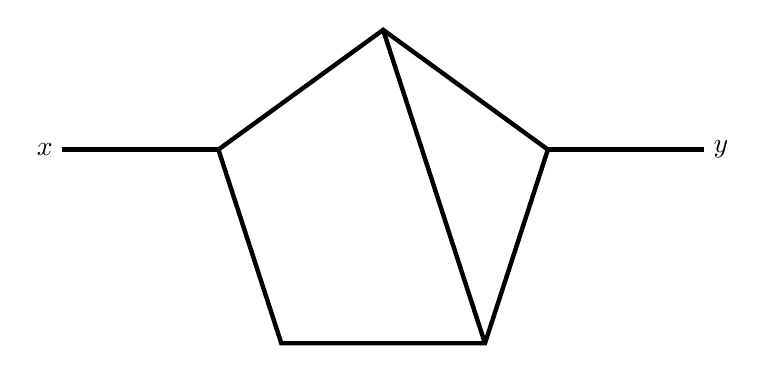
\begin{tikzpicture}[scale=2.2]%change the size here
	%pentagon
	\draw[ultra thick] (0,1)--(-0.9510565163,0.309017)--(-0.58778525229,-0.809017)--(0.58778525229,-0.809017)--(0.9510565163,0.309017)--cycle;
	%extra edges
	\draw[ultra thick] (0,1)--(0.58778525229,-0.809017);
	\draw[ultra thick] (-1.8510565163,0.309017)--(-0.9510565163,0.309017);
	\draw[ultra thick] (1.8510565163,0.309017)--(0.9510565163,0.309017);
	%label nodes   
	\node [left] at (-1.8510565163,0.309017) {$x$};
	\node [right] at (1.8510565163,0.309017) {$y$};
	\end{tikzpicture}
\end{center}

\begin{Exercise}[counter={sorszam}, difficulty=0]
	Azt mondjuk, hogy egy ir\'any\'itott %$G=(V,E)$
	gr\'af t\"om\"oren reprezent\'alt, ha adott egy $T$ Turing-g\'ep, ami $u,v$ bemenetre ki\'irja, hogy $uv$ \'el-e $\le n^k$ id\H oben, ahol $k$ egy fix konstans, pl.\ a feladat szempontj\'ab\'ol legyen $k=2$. A \la{Succinct-STconn} nyelv elemei azon $T$ Turing-g\'epek le\'ir\'asai, amik olyan gr\'afot t\"om\"or\'itenek, amiben van $st$ \'ut.\\
	a) Mutasd meg, hogy \PSPACE-ben eld\"onthet\H o \la{Succinct-STconn}.\\
	b) Mutasd meg, hogy \la{Succinct-STconn} \PSPACE-teljes.
\end{Exercise}	
\begin{Answer}
	a) \cl{NPSPACE}-beli \'es Savitch t\'etel.\\
	b) Az \'altal\'anos\'itott \'allapottere egy \PSPACE-es TG-nek pont egy ilyen gr\'afot ad.
\end{Answer}



\begin{Exercise}[counter={sorszam}, difficulty=2]
	a) A \la{Generalized Geography}-nak az a verzi\'oja is $\PSPACE$-teljes, ha a k\'et j\'at\'ekos k\"ul\"on-k\"ul\"on \'ep\'iti a saj\'at l\'anc\'at ugyanazon az ir\'any\'itott gr\'afon.
	(B\'armely cs\'ucsba csak egyik\"uk l\'ephet; mindkett\H onek meg van adva, hogy honnan kezd.)\\
	b) Ugyanez ir\'any\'itatlan gr\'afokra is $\PSPACE$-teljes.\\
	Mj.\ Azt nem tudom vizsg\'alt\'ak-e ezekben a verzi\'okban, hogy mi van, ha cs\'ucsokat szabad \'ujra haszn\'alni, csak az \'eleket nem.
\end{Exercise}	
\begin{Answer}
	Miltzow: Tron, a combinatorial Game on abstract Graphs \url{https://arxiv.org/abs/1110.3211} cikkben 13.~oldalt\'ol a), 15.\ oldalt\'ol b). (De egy\'ebk\'ent Nagy Kartal csin\'alt egyszer\H ubb megold\'ast r\'a.) 
\end{Answer}






\chapter{NP}



\begin{Exercise}[counter={sorszam}, difficulty=0]
	a) Mutasd meg, hogy \PSPACE-ben van a $3$-sz\'innel sz\'inezhet\H o gr\'afok nyelve.\\
	b) Mutasd meg, hogy \NP-ben van a $3$-sz\'innel sz\'inezhet\H o gr\'afok nyelve.\\
	c) Mutasd meg, hogy ha \P-ben van a $3$-sz\'innel sz\'inezhet\H o gr\'afok nyelve, akkor polinom id\H oben tudunk is keresni egy $3$-sz\'innel sz\'inez\'est.	
\end{Exercise}	
\begin{Answer}
	a) V\'egigpr\'ob\'algatjuk az \"osszes $3$-sz\'inez\'est, az aktu\'alis sz\'inez\'es le\'ir\'asa mindig csak $O(n)$ t\'ar, ellen\H orz\'eshez csak v\'egig kell menni az \'eleken.\\
	b) Tan\'u egy $3$-sz\'inez\'es.\\
	c) V\'egigmegy\"unk a nem-\'eleken \'es sorban hozz\'aadjuk a gr\'afhoz, amelyik nem rontja el a $3$-sz\'inezhet\H os\'eget. Ezt onnan tudjuk, hogy minden \'el hozz\'aad\'asa ut\'an ellen\H orizz\"uk, hogy a gr\'af $3$-sz\'inezhet\H o maradt-e. \'Igy v\'eg\"ul egy $3$-oszt\'aly\'u teljes gr\'afot kapunk, ezek lesznek a sz\'inoszt\'alyok.\\
	Fontos t\'ipushiba, hogy a $3$-sz\'inezhet\H os\'eg tesztel\H o algoritmusnak nem adhatunk olyan gr\'afot, aminek n\'eh\'any cs\'ucsa m\'ar ki van sz\'inezve!
\end{Answer}




\begin{Exercise}[counter={sorszam}, difficulty=0]
	a) Mutasd meg, hogy \NP-ben van, hogy egy gr\'afban van-e teljes p\'aros\'it\'as.\\
	b) Mutasd meg, hogy ha \P-ben van, hogy egy gr\'afban van-e teljes p\'aros\'it\'as, akkor polinom id\H oben tudunk is keresni egyet (ha van).\\
	c) Mutasd meg, hogy p\'aros gr\'afban tudunk teljes p\'aros\'it\'ast keresni polinom id\H oben.\\
	d)~\veryhard Mutasd meg, hogy \'altal\'anos gr\'afban is. (Persze lehet, hogy valaki m\'ar tanulta.)
\end{Exercise}	
\begin{Answer}
	a) Tan\'u egy teljes p\'aros\'itas.\\
	b) Egyes\'evel kit\"or\"olj\"uk az \'eleket \'es megn\'ezz\"uk, hogy van-e m\'eg teljes p\'aros\'it\'as. Ha nincs, akkor visszarakjuk az \'elet. \'Igy v\'eg\"ul egy teljes p\'aros\'it\'as \'elei maradnak.\\
	c) Opkutb\'ol tanult jav\'it\'outas m\'odszer ilyen.\\
	d) Edmonds-t\'etel: \url{https://en.wikipedia.org/wiki/Blossom_algorithm}.
\end{Answer}




\begin{Exercise}[counter={sorszam}, difficulty=0]
	Mutasd meg, hogy\\
	a) $\coNP$-beli,\\
	b)~\hard $\NP$-beli,\\
	c)~\veryhard $\P$-beli\\
	a Pr\'imek illetve a S\'ikbarajzolhat\'o gr\'afok nyelve.\\
	(Ez \"osszesen 6 feladat, van k\"ozt\"uk megoldhatatlanul neh\'ez is.)
\end{Exercise}	
\begin{Answer}
	a) Nem-pr\'ims\'egre tan\'u egy oszt\'o, nem s\'ikbelis\'egre egy felosztott $K_5$ vagy $K_{3,3}$ (Kuratowski-t\'etel miatt).\\
	b) Pr\'imekre 4.3.5. Tétel Lov\'asz k\"onyvben. S\'ikgr\'afokra t\'ipushiba, hogy a F\'ary t\'etel szerint van egyenes szakaszokkal is s\'ikbarajzol\'as \'es el\'eg a cs\'ucsok koordin\'at\'ait megadni, mert ez nem felt\'etlen\"ul \'irhat\'o le polinom helyen. Egy nem-trivi\'alis t\'etel, hogy minden gr\'af lerajzolhat\'o egy $2n\times n$ m\'eret\H u r\'acsra. Ehelyett egy egyszer\H u megold\'as, hogy topol\'ogiailag megadjuk, hogy mik a cs\'ucsokbol kimen\H o \'elek sorrendjei, melyik \'el melyik lapon van \'es a lapokon mi a sorrend. R\'eszletek meggondoland\'ok.\\
	c) Pr\'imekre ez nagyon sok\'aig nyitott volt, l\'asd \url{https://en.wikipedia.org/wiki/AKS_primality_test}. S\'ikgr\'afokra itt tal\'alhat\'ok k\"ul\"onb\"oz\H o megold\'asok: \url{https://cstheory.stackexchange.com/questions/24962/what-is-simplest-polynomial-algorithm-for-planarity}.
\end{Answer}



\begin{Exercise}[counter={sorszam}, difficulty=0]
	a) Mutasd meg, hogy $\DTIME(n^2)\ne\DTIME(n^{10})$.\\
	%lovasz 3.3.5-os tetel; 3.3.3 Tetelhez hasonloan, azaz univerzalis es atlos modszer.
	b)~\veryhard Mutasd meg, hogy $\NTIME(n^2)\ne\NTIME(n^{10})$.
\end{Exercise}	
\begin{Answer}
	a) Az id\H ohierarchia t\'etel miatty minden rekurz\'iv $f$-re van olyan rekurz\'iv nyelv, ami nincs $\DTIME(f(n))$-ben. A bizony\'it\'as r\'eszletein v\'egigmenve ellen\H orizhet\H o, hogy $f(n)=n^2$-re a kapott nyelv $\DTIME(n^{10})$-beli.\\
	b) Legegyszer\H ubb bizony\'it\'as Z\'ak: \url{http://blog.computationalcomplexity.org/2011/04/new-proof-of-nondeterministic-time.html}.
\end{Answer}



\begin{Exercise}[counter={sorszam}, difficulty=0]
	a) Mutasd meg, hogy van olyan $f$, amire minden rekurzív nyelv benne van a $\DTIME(f(n))$-ben.\\
	%lovasz 3.3.2-os tetel
	b)~\hard Mutasd meg, hogy van olyan rekurz\'iv $f$, amire $\DTIME(f(n))=\DTIME(2^{f(n)})$.
	%lovasz 3.3.6-os tetel
\end{Exercise}	
\begin{Answer}
	a) Vegy\"uk egy felsorol\'as\'at az \"osszes Turing-g\'epnek, ami mindig meg\'all: $T_1, T_2, \ldots$ \'es legyen $f(n)=\max_{i\le n}$ a $T_i$ l\'ep\'essz\'ama legfeljebb $n$ hossz\'u inputokon. Ha $L$ rekurz\'iv, akkor van egy $i$, hogy $L=L(T_i)$, teh\'at $L\in \DTIME(f(n))$.
	L\'asd m\'g \emph{busy beaver} f\"uggv\'eny.\\
	b) H\'ezag t\'etel: \url{https://en.wikipedia.org/wiki/Gap_theorem}.
\end{Answer}


\section{NP-teljess\'eg}


\begin{Exercise}[counter={sorszam}, difficulty=0]
	Adva van egy konjunktív normálforma. Szeretnénk eldönteni, hogy megválaszthatjuk-e úgy a változókat, hogy minden klóz tartalmazzon igaz és hamis literált is. Mutassuk meg, hogy annak eldöntése, hogy ezt lehet-e, \NP-teljes.
	%ez a halmazrendszer ketszinezhetoseg a spec esete.
	%NAE-SAT. minden klozhoz hozzaadjuk ugyanazt az uj valtozot. ha azt akarjuk, hogy minden klozban max 3 literal legyen, uugy megy klozok szetszedese, mint 3-SAT-nal.
\end{Exercise}	
\begin{Answer}
	\NP-belis\'eg nyilv\'anval\'o.
	Legegyszer\H ubb megold\'as \NP-neh\'ezs\'egre \'eszrevenni, hogy ez pont ugyanaz, mint a halmazrendszer k\'etsz\'inezhet\H os\'ege, ha egyik v\'altoz\'o sincs neg\'alva. Teh\'at mivel ez az \NP-teljes feladat a speci\'alis esete, ez\'ert ez is \NP-neh\'ez.
	De vissza lehetett vezetni a \SAT-ra is t\"obbf\'elek\'eppen; egyik opci\'o volt, hogy minden kl\'ozba betessz\"uk ugyanazt az \'uj v\'altoz\'ot, egy m\'asik meg, hogy minden kl\'ozb\'ol vesz\"unk m\'egegy p\'eld\'anyt, ahol minden v\'altoz\'ot neg\'alunk.
\end{Answer}



\begin{Exercise}[counter={sorszam}, difficulty=0]
	\NP-teljes, hogy egy $2n$ pont\'u gr\'afban van-e $n$-es klikk.
	%flenes dualisa, meg par izolalt (teljes foku) pont kell
	%vagy lehet az eloadason szerepelt konstrukcioval 3COL-bol.
\end{Exercise}	
\begin{Answer}
	\NP-belis\'eg nyilv\'anval\'o.
	Legegyszer\H ubb megold\'as \NP-neh\'ezs\'egre felhaszn\'alni, hogy \la{Independent}, azaz azt eld\"onteni, hogy van-e $k$ m\'eret\H u f\"uggetlen halmaz egy gr\'afban, \NP-teljes. T\'ipushiba, hogy $k=n$-et v\'alasztjuk visszavezet\'esnel, ezt azonban nem tehetj\"uk meg, mert $k$ az input r\'esze volt. Helyes megold\'as, hogy ha $(G,k)$ volt az input az \la{Independent}-nek, akkor abb\'ol \'ugy k\'esz\'it\"unk egy $G'$ gr\'afot, hogy $G$-nek vessz\"uk a komplementer\'et (hogy a f\"uggetlen halmazokb\'ol klikkek legyenek) \'es m\'eg hozz\'avesz\"unk $2k-n$ izol\'alt pontot, ha $2k\ge n$ (\'igy $k=(n+2k-n)/2$, azaz $k$ pont a $G'$ cs\'ucssz\'am\'anak a fele), illetve $n-2k$ pontot, akik mindenkivel \"ossze vannak k\"otve (\'igy $k+n-2k=(n+n-2k)/2$, azaz $n-k$ pont a $G'$ cs\'ucssz\'am\'anak a fele). Mindk\'et esetben akkor \'es csak akkor van $G'$-ben $|V(G')|/2$ m\'eret\H u klikk, ha $G$-ben volt $k$ f\"uggetlen pont.
	%Term\'eszetesen \'ugy is meg lehet oldani a feladatot, hogy az el\H oad\'asbeli visszavezet\'es l\'ep\'eseit m\'asoltuk le.
\end{Answer}


\begin{Exercise}[counter={sorszam}, difficulty=1]
	Mutasd meg, hogy annak eld\"ont\'ese, hogy egy gr\'afban van-e Hamilton-\'ut, \NP-teljes.
\end{Exercise}	
%\begin{Answer}
%\end{Answer}

\begin{Exercise}[counter={sorszam}, difficulty=0]
	Az el\H oz\H o feladatot felhaszn\'alva mutasd meg, hogy az al\'abbi feladatok is \NP-teljesek.\\
	a) Van-e a gr\'afban Hamilton-k\"or?\\
	b) Van-e a gr\'afban a cs\'ucsoknak legal\'abb a fel\'et tartalmaz\'o k\"or?\\
	c) \la{TSP}: Ha az \'eleken adott egy metrikus hosszf\"uggv\'eny (azaz a gr\'af teljes \'es teljes\"ul a hosszakra a h\'aromsz\"og egyenl\H otlens\'eg), van-e legfejlebb $K$ \"osszhossz\'u Hamilton-k\"or?
	%a ha eleket egyesevel adunk hozza, az tobb kerdes (Turing vagy Cook), ha egy n foku %csucsot, az egy kerdes (Karp), def eloadason utobbi volt!
	%b adjunk hozza n izolalt pontot egy grafhoz, igy el tudnank donteni H-kort.
	%c K=n es graf eleire 1, nem elekre 2-t irunk
\end{Exercise}	
\begin{Answer}
	\NP-belis\'eg nyilv\'anval\'o mindegyik esetben.\\
	a) A Hamilton-utat vezetj\"uk vissza. Vegy\"unk hozz\'a az input $G$ gr\'afhoz egy \'uj cs\'ucsot, akit mindenkivel \"osszek\"ot\"unk. \'Igy az \'uj gr\'afban akkor \'es csak akkor van Hamilton-k\"or, ha $G$-ben van Hamilton-\'ut.
	T\'ipushiba volt, hogy ha Hamilton-k\"or van, akkor Hamilton-\'ut is, teh\'at ez nehezebb. Gondolj\'atok meg, hogy ezzel a logik\'aval az is \NP-teljes lenne, hogy egy teljes gr\'af-e az input. Fontos, hogy a visszavezet\'esn\'el (l\'asd lap tetej\'en), akkor \'es csak akkor legyen az egyik input megold\'as az egyik feladatra, ha a m\'asik input is az a m\'asik feladatra.\\
	b) A Hamilton-k\"ort vezetj\"uk vissza. Vegy\"unk hozz\'a az input $G$ gr\'afhoz $|V(G)|$ izol\'alt pontot, vagy ak\'ar vegy\"uk $G$-t k\'et p\'eld\'anyban.\\
	c) A Hamilton-k\"ort vezetj\"uk vissza. Az input $G$ gr\'af \'eleire \'irjunk 1-et, a t\"obbi \'elre pedig 2-t \'es v\'alasszuk $K$-t $|V(G)|$-nek. \'Igy csak akokr van $n$ \"osszhossz\'u Hamilton-k\"or, ha $G$-ben volt Hamilton-k\"or. T\'ipushiba volt, hogy nem olvast\'atok el a z\'ar\'ojelben szerepl\H o felt\'eteleket...
\end{Answer}

\begin{Exercise}[counter={sorszam}, difficulty=0]
	Adott egy line\'aris egyenl\H otlens\'egrendszer.\\
	a) Mutassuk meg, hogy annak eldöntése, hogy van-e eg\'esz megold\'asa, \NP-neh\'ez.\\
	%mar az a spec eset, amikor 0\le xi\le 1 es sum xi>0 tipusuak is az, mert pont SAT.
	b)~\hard Mutassuk meg, hogy ez a feladat \NP-beli.
\end{Exercise}	
\begin{Answer}
	a) A \SAT egy inputj\'at k\"onny\H u \'at\'irni egyenl\H otlens\'egrendszerr\'e, de lehet sok m\'as dolgot is.\\
	b) Me\'g n\'eh\'any v\'altoz\'o hozz'aad\'as\'aval el\'erhet\H o, hogy $Ax=b, x\ge 0$ feladatot kelljen megoldani.
	Innen Cramer-szab\'aly meg egy\'eb dolgok kellenek, l\'asd: \url{http://lara.epfl.ch/web2010/_media/papadimitriou81complexityintegerprogramming.pdf}.
\end{Answer}

\begin{Exercise}[counter={sorszam}, difficulty=1]
	Mutasd meg, hogy \NP-teljes az $n^2$ elem\H u domin\'ok\'eszletek, amikkel lefedhet\H o egy $n\times n$-es n\'egyzet.
\end{Exercise}	
\begin{Answer}
	K\"ovetkezik abb\'ol, hogy b\'armely nemdeterminisztikus TG egy $n$ hossz\'u inputon ,,szimul\'alhat\'o'' egy domin\'o k\'eszlettel, amit egy determinisztikus TG el\H o tud \'all\'itani ismerve az inputot.
	Garant\'alhat\'o, hogy minden domin\'o csak egy helyre passzolhasson, ha mind megindexeljuk $(i,j)$-vel.
	Ezut\'an tudjuk egy TG fut\'as\'at szimul\'alni vel\"uk.
\end{Answer}

\begin{Exercise}[counter={sorszam}, difficulty=1]
	Annak eldöntése, hogy egy Sudokunak van-e megold\'asa, \NP-teljes. (Ha $n\times n$-es kisn\'egyzetek vannak.)
\end{Exercise}	



\begin{Exercise}[counter={sorszam}, difficulty=0]
	Jelölje $k$-SAT azon kielégíthet? konjunktív normálformák nyelvét, amelyekben minden klóz
	legfeljebb $k$ elem?, SAT-$k$ pedig azon konjunktív normálformákét, ahol minden változó legfeljebb $k$
	literálban fordul el?. Bizonyítsuk be (egyik volt el\H oad\'ason), hogy\\
	a) 2-SAT P-beli,\\
	b) 3-SAT NP-teljes,\\
	c) SAT-2 P-beli,\\
	d) SAT-3 NP-teljes.
\end{Exercise}	
\begin{Answer}
	a) A legfeljebb egy elem\H u kl\'ozokat irtsuk ki, am\'ig minden kl\'oz k\'etelem\H u nem lesz. Minden k\'etelem\H u kl\'oz le\'irhat\'o k\'et k\"ovetkeztet\'esk\'ent, pl.\
	$(x \vee y) \leftrightarrow (\bar x \to y) \leftrightarrow (\bar y \to x)$. Ez megad egy ir\'any\'itott gr\'afot a liter\'alokon, aminek k\'etszer annyi \'ele van, mint kl\'oz. Ha van olyan v\'altoz\'o, hogy a neg\'alt \'es a sima liter\'alja egy er\H osen \"osszef\"ugg\H o komponensben van, akkor nem megoldhat\'o a formula. Vegy\"uk \'eszre, hogy mivel a gr\'afot szimmetrikus m\'odon defini\'altuk, ez azzal ekvivalens, hogy nincs egyikb\H ol sem ir\'any\'itott \'ut a m\'asikba. Hasonl\'o okokb\'ol ekkor az is teljes\"ul, hogy nem lehet $x$-b\H ol ir\'any\'itott \'ut $y$-ba \'es $\bar y$-ba is. Viszont ilyenkor b\'armely v\'altoz\'onak v\'alaszthatunk tetsz\H olegesen \'ert\'eket, majd kit\"or\"olhetj\"uk az \'igy \'ert\'eket kapott v\'altoz\'okat, \'es ezt ism\'etelgethetj\"uk.\\
	b) Nagy kl\'ozokat sz\'etv\'agjuk kisebbekre, pl $(x_1\vee x_2\vee x_3\vee x_4) \leftrightarrow (x_1\vee x_2\vee y) \wedge (\bar y \vee x_3\vee x_4)$, ahol az $y$ egy \'uj v\'altoz\'o.\\
	c) A legfeljebb egyszer el\H ofordul\'o v\'altoz\'okat irtsuk ki, illetve azokat is, amiknek mindk\'et el\H ofordul\'asa neg\'alt vagy mindkett\H o sima. Tekints\"uk azt az ir\'any\'itatlan gr\'afot, aminek a cs\'ucsai a kl\'ozok \'es akkor van k\'et kl\'oz \"osszek\"otve, ha van k\"oz\"os v\'altoz\'ojuk. \'Igy a feladat ekvivalens azzal, hogy egy adott gr\'af \'elei megir\'any\'ithat\'oak-e \'ugy, hogy minden cs\'ucsba vezessen \'el. Ez visszavezethet\H o egy p\'aros\'it\'as feladatra p\'aros gr\'afban, ahol az egyik oszt\'alyban minden cs\'ucs foka 2.\\
	d) Szokott lenni el\H oad\'ason; Lov\'aszban 4.4.8. T\'etel.
\end{Answer}






\begin{Exercise}[counter={sorszam}, difficulty=0]
	Annak eldöntése, hogy term\'eszetes sz\'amok egy adott halmaz\'at sz\'et tudjuk-e osztani k\'et egyenl\H o r\'eszre, \NP-teljes.
\end{Exercise}	
\begin{Answer}
	A \la{SubsetSum} feladatot vezetj\"uk r\'a vissza, ahol azt kell megmondanunk, hogy input $a_i$ sz\'amok k\"oz\"ul van-e p\'ar, amiknek az \"osszege pont $b$. Az input sz\'amaink legyenek ugyanazok, valamint m\'egegy sz\'am, a $|2b-\sum_i a_i|.$
\end{Answer}


\begin{Exercise}[counter={sorszam}, difficulty=0]
	A \la{3DM} problémánál az input egy páros gráf, melyben a fels\H o osztályban minden pont foka $3$. Az alsó osztály három színnel van színezve, minden fels\H o osztálybeli pontnak minden színezett részbe egy éle megy. A kérdés, hogy létezik-e olyan ,,teljes alulról bepárosítás", hogy alul mindenkinek egy, felül mindenkinek $0$ vagy $3$ a foka. Mutassuk meg, hogy \la{3DM} \NP-teljes.\\
	(A feladat egy ekvivalens megfogalmaz\'asa, hogy adott egy h\'arom sz\'innel sz\'inezett alaphalmaz \'es rajta egy $3$-uniform hipergr\'af. A c\'el egy teljes p\'aros\'it\'as keres\'ese, ahol az \'elek most ugye h\'arom elem\H uek.)
\end{Exercise}	
\begin{Answer}
	Visszavezet\'es a \la{3-SAT}-r\'ol: Minden v\'altoz\'onak feleljen meg $k$ piros, $k$ k\'ek \'es $2k$ z\"old pont, mely ut\'obbiak legyenek sz\'etosztva k\'et $k$ elem\H u r\'eszre: $Z_x$-re \'es $Z_{\bar x}$-re. Adjunk meg ezen a $4k$ ponton halmazokat \'ugy, hogy a piros \'es k\'ek pontok egy teljes p\'aros\'it\'asa eset\'en vagy pontosan $Z_x$ vagy pontosan $Z_{\bar x}$ van fedve. Minden kl\'oznak feleljen meg egy piros \'es egy k\'ek pont, amik ugyanabban a h\'arom halmazban vannak benne, ahol a harmadik pontok a kl\'ozban lev\H o liter\'aloknak felelnek meg. V\'eg\"ul vegy\"unk fel m\'eg egy csom\'o piros \'es k\'ek pontot, hogy ne legyen baj a kimarad\'o z\"oldekkel.
\end{Answer}



\begin{Exercise}[counter={sorszam}, difficulty=1]
	A \la{Planar*-3SAT} problémánál adott egy s\'ikbeli páros gráf, melynek csúcsai egy konjuktív normál\-for\-mu\-la klózainak és változóinak felelnek meg, két csúcs akkor van összekötve, ha a változó szerepel a klózban. Mutassuk meg, hogy annak eldöntése, hogy igazz\'a tehet\H o-e, \NP-teljes.
\end{Exercise}	
\begin{Answer}
	Lichteinstein t\'etele.
\end{Answer}



\begin{Exercise}[counter={sorszam}, difficulty=0]
	Mutasd meg, hogy s\'ikgr\'afra  meghat\'arozni a kromatikus sz\'am\'at\\
	a)~\hard \NP-teljes,\\
	b) de h\'aromsz\"ogelt s\'ikgr\'afra \P-beli.
\end{Exercise}	
\begin{Answer}
	a)  L. Stockmeyer, Planar 3-colorability is polynomial complete. ACM SIGACT News 5 (1973),
	19--25.\\
	b) Tetsz\H oleges szomsz\'edos cs\'ucsokat kisz\'inez\"unk, majd vesz\"unk egy \'elet, aminek mindk\'et v\'ege ki van sz\'inezve, de a harmadik nincs, \'es azt is kisz\'inezz\"uk.
	De van egy egyszer\H u karakteriz\'aci\'o is: Akkor lesz 3-sz\'inezhet\H o egy h\'aromsz\"ogelt s\'ikgr\'af, ha nincs p\'aratlan fok\'u cs\'ucsa. Ezt \'ugy lehet bizony\'itani, hogy ha minden fok p\'aros, akkor a legkisebb fok 2 vagy 4 \'es innen indukci\'o. A 2 fok\'u eset trivi. Ha $v$ 4 fok\'u, akkor van k\'et szomsz\'edja, pl.\ $u$ \'es $w$, amik nem szomsz\'edosak egym\'assal. \"Osszeh\'uzzuk az $u,v,w$ cs\'ucsokat egy cs\'uccs\'a, indukci\'oval sz\'inezz\"uk ezt a gr\'afot. A foksz\'am-felt\'etel miatt $v$ m\'asik k\'et eredeti szomsz\'edja ugyanazt a sz\'int fogja kapni, \'ugyhogy a sz\'eth\'uz\'asn\'al $u$ \'es $w$ \H orizze meg a sz\'in\'et, m\'ig $v$ kaphatja a harmadik sz\'int.
	%https://faculty.math.illinois.edu/~west/pubs/eultri.pdf
\end{Answer}


\begin{Exercise}[counter={sorszam}, difficulty=0]
	Egy $G$ gr\'af \emph{f\'elkromatikus sz\'ama} az a legkisebb $k$, amire $G$ cs\'ucsainak fel\'et lehet \'ugy $k$-sz\'inezni, hogy b\'armely k\'et szomsz\'edos cs\'ucs m\'as sz\'int kapjon. (Cs\'ucsok m\'asik fele sz\'inezetlen maradhat.) Mutasd meg, hogy \NP-teljes eld\"onteni, hogy egy gr\'af f\'elkromatikus sz\'ama 3-e.
\end{Exercise}	
\begin{Answer}
	Ha $G$ a \la{3col} inputja, akkor csin\'aljunk bel\H ole $G'$-t \'ugy, hogy hozz\'avesz\"unk $|V(G)|$ cs\'ucsot, akik mindenkivel \"ossze vannak k\"otve.
\end{Answer}

\bigskip
\defi Egy halmazrendszer/hipergr\'af (cs\'ucsainak) $k$-sz\'inez\'es\'et t\"obbf\'elek\'eppen defini\'alhatjuk.\\
a) (gyenge) $k$-sz\'inez\'es: minden hiper\'elben szerepeljen k\'et k\"ul\"onb\"oz\H o sz\'in.\\
b) sziv\'arv\'any $k$-sz\'inez\'es: minden hiper\'elben minden sz\'in k\"ul\"onb\"oz\H o legyen.\\
c) konfliktusmentes $k$-sz\'inez\'es: minden $e$ hiper\'elben szerepeljen egy cs\'ucs, aminek a sz\'ine az \"osszes t\"obbi $e$-beli sz\'int\H ol k\"ul\"onb\"oz\H o.\\
d) polikromatikus $k$-sz\'inez\'es: minden hiper\'elben szerepeljen mind a $k$ sz\'in.

\begin{Exercise}[counter={sorszam}, difficulty=0]
	Mutasd meg, hogy mind a n\'egy verzi\'o \NP-teljes minden $k\ge 3$ konstansra.
\end{Exercise}	
\begin{Answer}
	a-b-c) Ezek sima gr\'afokra pont ugyanazok, mint a $k$-sz\'inezhet\H os\'eg, $k$-\la{col}.\\
	d) Ha $G$ a $k$-\la{col} inputja, akkor legyen $\HH$ az  hipergr\'af, hogy $G$ minden \'el\'ehez hozz\'aadunk $k-2$ \'uj cs\'ucsot.
%a)-ra ez is jo: Ha $\HH$ a \la{2col} inputja, akkor legyen $\HH'$ cs\'ucshalmaza $V(\HH)\dot\cup K$, ahol $K$ $k$ db \'uj cs\'ucs, $\HH'$ \'elei pedig legyenek $\binom K2\cup \{E(\HH)+\binom K1\}$, azaz $K$ k\'etelem\H u r\'eszhalmazai, valamint $\HH$ \'elei kieg\'esz\'itve egy darab $K$-beli cs\'uccsal, az \"osszes lehets\'eges m\'odon.
\end{Answer}

\begin{Exercise}[counter={sorszam}, difficulty=0]
	Mutasd meg, hogy $k$-uniform hipergr\'afokra is \NP-teljesek minden $k\ge 3$ konstansra.
\end{Exercise}	
\begin{Answer}
	b-d) Ezekre j\'o az el\H oz\H o feladatbeli visszavezet\'es.\\
	a) Ha $G$ a $k$-\la{col} inputja, akkor legyenek a $\HH$ hipergr\'af cs\'ucsai $V(G)\dot\cup W$, ahol $W$ $k(k-1)$ db \'uj cs\'ucs, $\HH$ \'elei pedig legyenek $\binom Wk\cup \{E(G)+\binom W{k-2}\}$, azaz $W$ $k$-elem\H u r\'eszhalmazai, valamint $G$ \'elei kieg\'esz\'itve $k-2$ darab $W$-beli cs\'uccsal, az \"osszes lehets\'eges m\'odon.\\
	c) Ugyanaz, mint a)-ra, csak \'elhalmaz kisebb, csak $E(G)+\binom W{k-2}$-b\H ol \'all.
\end{Answer}


\begin{Exercise}[counter={sorszam}, difficulty=2]
	Annak eldöntése, hogy egy kvadratikus diophantoszi egyenletnek van-e
	megold\'asa, \NP-teljes.
\end{Exercise}	
\begin{Answer}
	\url{http://cstheory.stackexchange.com/questions/14124/is-there-a-natural-problem-on-the-naturals-that-is-np-complete/14147#14147}.
\end{Answer}


\begin{Exercise}[counter={sorszam}, difficulty=1]
	Egy $n$ r\'esztvev\H os focibajnoks\'agot $k$ fordul\'o ut\'an le kellett \'all\'itani a koronav\'irus miatt.\\
	a)~\veryhard (nem ismert) \NP-teljes-e input tabella alapj\'an eld\"onteni, hogy egy csapat lehet-e m\'eg bajnok?\\
	b)~\hard Ha az is az input r\'esze, hogy ki kivel j\'atszott, akkor \NP-teljes.
\end{Exercise}	
\begin{Answer}
	b) Walter Kern, Dani\"el Paulusma,
	The new FIFA rules are hard: complexity aspects of sports competitions,
	Discrete Applied Mathematics 108 (3),
	2001, 317--323, \url{https://doi.org/10.1016/S0166-218X(00)00241-9}.
\end{Answer}





\chapter{PAD}

\defi $PAD(L)=\{x0^{n^2}:x\in L\}$ (azaz $x$ mögé írunk még egy csomó nullást és persze $n=|x|$).

\begin{Exercise}[counter={sorszam}, difficulty=0]
	Mutassuk meg, hogy $\DTIME(n)\ne \DTIME(n^{1.01})\ne \DTIME(n^2)\ne \DTIME(n^{2.01})$.
\end{Exercise}	
%\begin{Answer}
%\end{Answer}


\begin{Exercise}[counter={sorszam}, difficulty=0]
	Ha $\P=\NP$, akkor $\EXP=\NEXP$.
\end{Exercise}	
\begin{Answer}
	$PAD$-eljunk. Indirekt tegy\"uk fel, hogy van $L$ $\NEXP\setminus \EXP$-ben. Ekkor ez benne van valamilyen $k$-ra $\NTIME(2^{n^k})$-ben. $PAD$-elj\"uk meg $2^{n^k}$ darab null\'aval. Ekkor $PAD(L)$ m\'ar \NP-beli, teh\'at \P-beli is, teh\'at $L\in \EXP$, ellentmond\'as.
\end{Answer}

\begin{Exercise}[counter={sorszam}, difficulty=0]
	$\P\cap\TALLY=\NP\cap\TALLY \Longleftrightarrow\E=\NE$.\\ (\TALLY-val jelöljük az egybet\H us nyelvek osztályát, $\E=\DTIME(2^{O(n)})$ \'es $\NE=\NTIME(2^{O(n)}$.)
\end{Exercise}	
%\begin{Answer}
%\end{Answer}

\begin{Exercise}[counter={sorszam}, difficulty=0]
	Ha $\E=\NE$, akkor nincs ritka nyelv $\NP\setminus \P$-ben. Azaz ha $\DTIME(2^{O(n)})=\NTIME(2^{O(n)})$, akkor ha egy $L\in \NP$ nyelvben minden $n$-re az $n$ hossz\'u szavak sz\'ama $O(n^c)$, akkor $L\in \P$.
\end{Exercise}	
\begin{Answer}
	Legyen $L'=\{(n,k,l,i,b)\mid \textit{van k darab n hossz\'u L-beli sz\'o \'ugy, hogy az l.\ sz\'o i.\ bitje b}\}$.
	Ha $L\in \NP$, akkor $L'\in \NE$, mert nemdeterminisztikusan felsorolhatjuk a $k$ darab $n$ hossz\'u sz\'ot, $L\in \NP$ seg\'its\'eg\'evel mindre tudunk tan\'ut is tal\'alni.
	A feltev\'es szerint ekkor $L'\in \E$ is teljes\"ul.
	Most ezt felhaszn\'alva megmutatjuk, hogy $L\in \P$.
	Bin\'aris keres\'essel megtal\'aljuk azt a legnagyobb $k$-t, amire $(n,k,1,1,0)\in L'$ vagy $(n,k,1,1,1)\in L'$; ez lesz az $n$ hossz\'u szavak sz\'ama $L$-ben.
	Ezut\'an minden $l\le k$, $i\le n$, $b=0/1$ h\'armasra megn\'ezz\"uk, hogy $(n,k,l,i,b)$ benne van-e $L'$-ben.
	\'Igy mind a $k$ $L$-beli sz\'ot meghat\'aroztuk.
	%forras: https://cstheory.stackexchange.com/questions/47963/if-sfe-sfne-then-sfnp-p-contains-no-sparse-sets
\end{Answer}


\begin{Exercise}[counter={sorszam}, difficulty=0]
	$\NP\neq \E:= \DTIME(2^{O(n)})$.
\end{Exercise}	
%\begin{Answer}
%\end{Answer}







\chapter{Polinomi\'alis hierarchia \'es or\'akulumok}

\defi $\exists^p L := \left\{ x \in \{0,1\}^* \ \left| \ \left( \exists w \in \{0,1\}^{\leq p(|x|)} \right) \langle x,w \rangle \in L \right. \right\},$

\noindent
\'es hasonl\'oan $\forall^p L := \left\{ x \in \{0,1\}^* \ \left| \ \left( \forall w \in \{0,1\}^{\leq p(|x|)} \right) \langle x,w \rangle \in L \right. \right\}.$

\noindent
Ezekkel a jelölésekkel $\NP=\cl{\exists\cdot \P}$ és $\coNP=\cl{\forall\cdot \P}$. Ezen felbuzdulva $\Sigmak:=\cl{\exists\cdot\forall\cdot\exists\ldots \P}$ és $\Pik:=\cl{\forall\cdot\exists\cdot\forall\ldots \P}$, ahol összesen $k$ db kvantor áll a $\P$ el\H ott. Teh\'at ezekkel a jelölésekkel $\NP=\Sigmaone$ és $\coNP=\Pione$.
A polinomi\'alis hierarchia $\PH:=\cup \Sigmak$.
%Szint\'en elterjedt az $\MA=\cl{\exists\cdot \BPP}$ jel\"ol\'es.
%nem is uaz: https://complexityzoo.uwaterloo.ca/Complexity_Zoo:E#existsbpp

\begin{Exercise}[counter={sorszam}, difficulty=0]
	$\Sigmak\subset \Sigmakplus\cap\Pikplus$.
\end{Exercise}

\begin{Exercise}[counter={sorszam}, difficulty=0]
	$\Sigmak\subset\PSPACE$.
\end{Exercise}	

\begin{Exercise}[counter={sorszam}, difficulty=0]
	$\Pik\subset\Sigmak \Rightarrow \Sigmak=\PH$.
\end{Exercise}	

\begin{Exercise}[counter={sorszam}, difficulty=0]
	Tegy\"uk fel, hogy adva van egy konjukt\'iv norm\'al forma, melynek v\'altoz\'oi $x_i$-k \'es $y_i$-k. Azt szeretn\'enk eld\"onteni, hogy minden $x_i$ behelyettes\'it\'esre van-e az $y_i$-knek olyan behelyettes\'it\'ese, ami kiel\'eg\'it\H o. Mutassuk meg, hogy ez $\Pitwo$-ben van. Mi lenne, ha az lenne a k\'erd\'es, hogy van-e $x_i$, hogy minden $y_i$-re igaz a formula?
\end{Exercise}	 
\begin{Answer}
	Akkor trivin \Sigmatwo-ban lenne, de az is igaz, hogy \NP-beli, mert azt k\"onny\H u ellen\H orizni, hogy egy KNF-et minden \'ert\'ekad\'as igazz\'a tesz-e.
\end{Answer}

\begin{Exercise}[counter={sorszam}, difficulty=0]
	Legyen $L$ az $n^2\times n^2$ m\'eret\H u olyan \'altal\'anos\'itott Sudoku \'all\'asok nyelve, ahol ak\'arhova be\'irunk egy sz\'amot (nem azonos sorba/oszlopba/n\'egyzetbe egy ugyanolyan sz\'ammal), marad megold\'asa.\\
	a) Melyik oszt\'alyban van $L$?\\
	b) Nincs benne egy kisebben is?
\end{Exercise}	
\begin{Answer}
	\Pitwo-ban van trivi, de igaz\'ab\'ol \Sigmaone-ben is, mert az \"osszes lehet\H os\'eget leellen\H orizhetj\"uk.
\end{Answer}

\begin{Exercise}[counter={sorszam}, difficulty=1]
	$\NP \subset \Ppoly \Rightarrow \Sigmatwo=\PH$.
\end{Exercise}	
\begin{Answer}
	Karp-Lipton t\'etel.\\
	\"Otlet: El\H oször mutassuk meg, hogy ekkor olyan hálózat is van, ami minden kielégíthet\H o \SAT formulához ad egy helyes kiértékelést. Aztán mutassuk meg, hogy \"osszeomlana a polinomi\'alis hierarchia.
	
	Ha $\NP \subset \Ppoly$, akkor van egy $p(n)$ poly hossz\'u bitsorozat \'es $T$ TG, hogy $T(\Psi,p(n))=1$ akkor \'es csak akkor ha $\Psi\in\SAT$. S\H ot, olyan $T$ is van, hogy $T(\Psi,p(n))=1$ eset\'en m\'eg ki is ad egy $x$-et, amire $\Psi(x)$ igaz. Most azt fogjuk megmutatni, hogy $\Pitwo\subset\Sigmatwo$, ebb\H ol k\"ovetkezik az \'allit\'as. Legyen $L\in \Pitwo$. Ekkor $\Psi\in L$ akkor \'es csak akkor, ha minden $z$-re $\Psi_z\in \SAT$, valami \P-beli $\Psi_z$-re. De ez ekvivalens azzal, hogy $\exists p(n) \forall z T(\Psi_z,p(n))=1$ \'es $\Psi_z(x_z)$ igaz, ahol az $x_z$-t is $T$ adja ki.
\end{Answer}

\begin{Exercise}[counter={sorszam}, difficulty=1]
	$\EXP\subset \Ppoly \Rightarrow \EXP= \Sigmatwo$.
\end{Exercise}	
\begin{Answer}
	Meyer t\'etele (de Karp-Lipton cikkben van).\\
	El\H oz\H oh\"oz hasonl\'oan. Lenne egy hálózat, ami egy \EXP-es sz\'am\'it\'as b\'armelyik hely\'en, b\'armikor felvett \'ert\'eket meg tudn\'a mondani. Egy ilyennek a helyess\'eg\'et ellen\H orizni is tudjuk \coNP-ben.
	%forras: vargadanis
\end{Answer}

\begin{Exercise}[counter={sorszam}, difficulty=0]
	Tegyük fel, hogy adott egy játék, ahol két játékos felváltva lép és egy $poly(n)$ méret\H u táblán játszanak \'ugy, hogy felv\'altva elfoglalnak egy mez\H ot (pl.\ am\H oba). Az állás alapján mindig el lehet dönteni \P-ben, hogy nyert-e valaki. Tegy\"uk fel, hogy a játék $k$ lépés alatt garant\'altan véget ér. Mutassuk meg, hogy azon \'all\'asok nyelve, amikre kezd\H onek van nyer\H o stratégiája $\in \Sigmak$. S\H ot.
\end{Exercise}	
\begin{Answer}
	S\H ot (Borb\'enyi M\'arton), \P-beli, mert csak ennyi opci\'o van konstans k\"or\"os j\'at\'ekban \'es mindet v\'egign\'ezhetj\"uk.
	Ha a t\'abla exp m\'eret\H u lenne vagy k\"or\"onk\'ent $n$-et rakn\'anak, akkor csak \Sigmak-t tudn\'ank bizony\'itani.	
\end{Answer}

%\pro A bemenet legyen $n$ db $n$-edfok\'u polinom (nem felt\'etlen\"ul standard form\'aban megadva, lehetnek t\"obbv\'altoz\'osak is), a c\'el eld\"onteni, hogy van-e egy nem \"ures r\'eszhalmazuk, aminek az \"osszege azonosan nulla. Mutassuk meg, hogy ez $\MA$-ban van.
%miutan megmondjak melyik, mar le tudjuk tesztelni a schwartz lemmaval

\bigskip
\defi Az {\em orákulumos} Turing-gép egy többszalagos $M^?$ Turing-gép, melynek egyik szalagja a kitüntetett kérdez\H o-szalag. Az orákulum egy tetsz\H oleges $A$ nyelv lehet. $M^?$-nek van egy speciális $q_?$ állapota. Ha ebbe kerül, akkor az orákulum válaszol neki, hogy az éppen akkor a speciális szalagján lev\H o szó benne van-e az $A$ nyelvben. 

Az $x$ bemenethez tartozó kimenetet $M^A(x)$-szel jelöljük. Ha $\XP$ egy olyan nyelv, ami Turing-gépek egy speci\'alis családj\'aval van defini\'alva, akkor $\XP^A$ jelöli azokat az $L$ nyelveket, amihez van ebb\H ol a csal\'adb\'ol Turing-g\'ep, amihez $A$ orákulumot adva $L$-et ismeri fel. Ha valamely bonyolults\'agi oszt\'alyhoz van teljes nyelv, akkor gyakran a bonyolults\'agi oszt\'alyt \'irjuk a kitev\H obe, pl. $\P^{\NP}$ azt jelenti, hogy $\P^{\SAT}$. Ha nincs teljes nyelv, akkor is \'irhatunk bonyolults\'agi oszt\'alyt a kitev\H obe, ekkor az \'uj oszt\'aly az \"osszes lehets\'eges nyelv uni\'oja, pl.\ $\P^{\BPP}=\cup \{\P^{L}\mid {L\in \BPP}\}$.

\begin{Exercise}[counter={sorszam}, difficulty=0]
	Legyen $A$ egy $\P$-beli nyelv. Mutassuk meg, hogy $\P^A=\P$.
\end{Exercise}	
\begin{Answer}
	Futassuk magunk az $A$-t eld\"ont\H o TG-et ahelyett, hogy k\'erdezn\'enk t\H ole.
\end{Answer}


\begin{Exercise}[counter={sorszam}, difficulty=0]
	$\P^{\NP}=\P^{\SAT}$.
\end{Exercise}	
\begin{Answer}
	Minden \NP-beli nyelv visszavezethet\H o \SAT-ra, \'es azt\'an mint el\H oz\H o.
\end{Answer}


\begin{Exercise}[counter={sorszam}, difficulty=0]
	Ha $\E=\DTIME(2^{O(n)})$, akkor mi lesz $\P^{\E}$?
\end{Exercise}	
\begin{Answer}
	\EXP.
\end{Answer}


\begin{Exercise}[counter={sorszam}, difficulty=0]
	$\PSPACE^{\PSPACE}=\PSPACE$.
\end{Exercise}	
%\begin{Answer}
%\end{Answer}


\begin{Exercise}[counter={sorszam}, difficulty=0]
	Mutasd meg, hogy $\NP\cup \coNP\subset \P^{\NP}$.
\end{Exercise}	
\begin{Answer}
	$\NP\subset \P^{\NP}$ nyilv\'anval\'o \'es $\P^{\NP}$ z\'art komplementerre.
\end{Answer}


\begin{Exercise}[counter={sorszam}, difficulty=0]
	$\NP^{\NP\cap \coNP}= \NP$.
\end{Exercise}	
\begin{Answer}
	B\'armit k\'erdezn\'enk, megtippelhetj\"uk r\'a a v\'alaszt \'es tal\'alhatunk r\'a tan\'ut magunk.\\
	Forr\'as: \url{http://blog.computationalcomplexity.org/2017/03/np-in-zpp-implies-ph-in-zpp.html} alapj\'an.
\end{Answer}


\begin{Exercise}[counter={sorszam}, difficulty=0]
	$\NP^{\NP}= \Sigmatwo$.
\end{Exercise}	
\begin{Answer}
	$\NP^{\NP}\supset \Sigmatwo$ defin\'ici\'o szerint.
	$\NP^{\NP}\subset \Sigmatwo$-hez tippelj\"uk meg \"osszes k\'erd\'esre v\'alaszokat, amire van tan\'u, tippelj\"uk meg, amire nincs, azokra meg ez egyetlen $\Pione$-beli mondat, hogy egyikhez sincs.
\end{Answer}

\begin{Exercise}[counter={sorszam}, difficulty=1]
	$\BPP^{\BPP}=\BPP$.
\end{Exercise}	
\begin{Answer}
	Legyen or\'akulumos TG fut\'asideje $n^k$ \'es hib\'azzon $<1/8$ es\'ellyel.
	Or\'akulum nyelvhez minden $n$-re \'es $k$-re van \BPP alg, ami $<1/(8n^k)$ es\'ellyel hib\'azik.
	Ez ism\'etelget\'essel kaphat\'o b\'armelyik \BPP-sb\H ol, teh\'at tudjuk is szimul\'alni $poly(n^k)$ id\H oben.
	Ha mindig ezt futtatjuk k\'erdez\'es helyett, akkor annak az es\'elye, hogy valaha is hib\'azunk k\'erdeze\'s szimul\'al\'asakor $<1/8$, teh\'at az \"osszhiba $<1/4$.
\end{Answer}


\begin{Exercise}[counter={sorszam}, difficulty=0]
	Mutass olyan $\XP$ bonyolults\'agi oszt\'alyt, amire $\XP^{\XP}\ne \XP$.
\end{Exercise}	
\begin{Answer}
	I. $\E$ vagy $\EXP$ j\'o id\H ohierarchia miatt.\\
	II. (Csern\'ak Tam\'as) Rekurz\'iv felsorolhat\'ok is j\'ok, mert nem z\'artak komplementerre.
\end{Answer}


\begin{Exercise}[counter={sorszam}, difficulty=0]
	$\exists A: \P^A= \NP^A$.
\end{Exercise}	
\begin{Answer}
	I. Ha $A$ \PSPACE-teljes, ez Savitch t\'etel.\\
	II. (\'Agoston P\'eter) $A=\PH$, mert ha nemdet $k$. szintr\H ol k\'erdez, det k\'erdezhet a $(k+1)$-edikr\H ol.
\end{Answer}


\begin{Exercise}[counter={sorszam}, difficulty=1]
	$\exists A: \P^A\ne \NP^A$.
\end{Exercise}	
\begin{Answer}
	Nyelv legyen, hogy van-e $A$-ban az inputtal megegyez\H o hossz\'us\'ag\'u string.
	Meg lehet csin\'alni \'atl\'os m\'odszerrel, hogy minden $\P$-belit\H ol k\"ul\"onb\"ozz\"on.
\end{Answer}


\begin{Exercise}[counter={sorszam}, difficulty=1]
	Van $A$ nyelv, hogy minden $L\in \NEXP^A$-hoz van $S\subset \N$ v\'egtelen halmaz \'es $L'\in\NP^A$, amire $L|_S=L'|_S$.
\end{Exercise}	
\begin{Answer}
	Forr\'as: Buhrman, Fortnow, Santhanam: Unconditional Lower Bounds Against Advice \url{https://doi.org/10.1007/978-3-642-02927-1_18}.
\end{Answer}






\chapter{V\'eletlen}

\begin{Exercise}[counter={sorszam}, difficulty=0]
	Adj egy (RAM g\'epen) $\tilde O(n^2)$ idej\H u randomiz\'alt algoritmust, ami eld\"onti input $A,B,C$ $n\times n$-es eg\'esz m\'atrixokr\'ol, hogy $A\cdot B=C$ igaz-e. Melyik oszt\'alyban van ez az algoritmus \RP, \coRP \'es \BPP k\"oz\"ul?
\end{Exercise}	
\begin{Answer}
	$AB=C$ akkor \'es csak akkor, ha minden $x$-re $A(Bx)=Cx$, teh\'at ez val\'oj\'aban egy $n$ v\'altoz\'os line\'aris polinomazonoss\'ag tesztel\'es.
	Konkr\'etan egy v\'eletlen $x\in \{0,1\}^n$-re tesztelj\"uk, hogy $A(Bx)=Cx$ igaz-e.
	Ha $AB=C$, ez mindig teljes\"ul.
	K\"ulonben legyen $(AB)_{ij}\ne C_{ij}$.
	Ekkor csak egy $x_j$ \'ert\'ekre lesz $(A(Bx)_i=(Cx)_i$.
	Teh\'at legal\'abb $1/2$ es\'ellyel $A(Bx)\ne Cx$.
	Ez egy \coRP-beli algoritmus, teh\'at \BPP-beli is.
\end{Answer}



\begin{Exercise}[counter={sorszam}, difficulty=0]
	Eld\"onthetelen egy le\'ir\'as\'aval adott randomiz\'alt, polinom id\H oben fut\'o Turing-g\'epr\H ol, hogy igaz-e, hogy
	minden $x$-et vagy legal\'abb $1/2$ es\'ellyel elfogad, vagy biztosan elutas\'it.
\end{Exercise}	
\begin{Answer}
	A meg\'all\'asi probl\'em\'at vezetj\"uk vissza.
	Input $T$-b\H ol k\'esz\'it\"unk egy $T'$-t, ami minden $x$ inputra $T$-t szimul\'alja a \"ures inputon $|x|$ l\'ep\'esig.
	Ha $T$ nem \'all le ezalatt, akkor $T'$ elutas\'it.
	Ha $T$ le\'all, akkor $T'$ fogadja el $|x|$-et $1/4$ es\'ellyel.
\end{Answer}


\begin{Exercise}[counter={sorszam}, difficulty=0]
	Mutasd meg p\'eld\'aul a \BPP -r\H ol, hogy ekvivalens defin\'ici\'okat kapunk, ha\\
	a) racion\'alis sz\'amok az eloszl\'asok (amik meghat\'arozz\'ak, hogy mikor merre l\'ep\"unk tov\'abb),\\
	b) csak egy darab \'allapot van, ami $1/2$--$1/2$ es\'ellyel l\'ep k\'et m\'asikba,\\
	c) van egy v\'eletlen szalagunk, melynek minden mez\H oje $1/2$ es\'ellyel 0 \'es 1,\\
	d) egy olyan p\'enzt ,,dob\'alhatunk'', ami valamilyen ismeretlen, konstans $p$ es\'ellyel lesz fej.
	%racokat jol kell kozeliteni, input hoszatol fuggoen
\end{Exercise}	
\begin{Answer}
	A b) az a) speci\'alis esete.\\
	Ha van egy a) t\'ipus\'u $T$ g\'ep\"unk, akkor abb\'ol \'ugy k\'esz\'ithet\"unk egy b) t\'ipus\'u $T'$-t, hogy ah\'anyszor randomiz\'alni kell, mindig le\'irjuk egy plusz szalagra, hogy \'eppen $T$ melyik \'allapot\'aban kell ezt megtenn\"unk, majd $T'$ egyetlen randomiz\'alt \'allapot\'aval addig sorsolunk, am\'ig el\'eg nagy pontoss\'aggal meg nem k\"ozel\'itj\"uk a racion\'alis sz\'amokat.
	A k\"ozel\'it\'es sz\"uks\'eges pontoss\'ag\'at, azaz azt, hogy a racion\'alis sz\'amot h\'any bin\'aris ``tizedes jegy'' pontoss\'agig sz\'amoljuk ki, az input hossza hat\'arozza meg.
	Ha $T$ $n^c$ id\H oben fut, akkor el\'eg $1/(2n^c)$ pontoss\'aggal k\"ozel\'iteni, \'igy az ebb\H ol ad\'od\'o hiba legfeljebb $(1-1/(2n^c))^{n^c}<1/e^2$, teh\'at az \"osszhiba legfeljebb $1/3+1/e^2<1/2$.
	Ez ism\'etl\'essel levihet\H o $1/3$ al\'a a szok\'asos m\'odon.\\
	A b) \'es c) ekvivalenci\'aja nyilv\'anval\'o.\\
	A d) speci\'alis esete a b)-c).\\
	Ha van egy b) t\'ipus\'u $T$ g\'ep\"unk, akkor abb\'ol \'ugy k\'esz\'ithet\"unk egy d) t\'ipus\'ut, hogy ah\'anyszor a randomiz\'al\'o \'allapotba l\'epn\'enk, dobjuk fel a p\'enzt k\'etszer.
	Ha fej-\'iras, l\'epj\"unk tov\'abb az egyik \'allapotba, ha \'iras-fej, akkor a m\'asikba, m\'ig ha k\'et azonos \'ert\'eket kapunk, akkor ism\'etelj\"uk ezt meg \'ujra.
	(Ha ezt olyan sokszor k\'ene megism\'etelni, hogy t\'ulmenn\'enk a megengedett fut\'asid\H on, akkor \'alljunk le, ennek \'ugyis kicsi az es\'elye.)
\end{Answer}

\begin{Exercise}[counter={sorszam}, difficulty=1]
	Mutasd meg, hogyha az eloszl\'asr\'ol csak azt tessz\"uk fel, hogy rekurz\'iv,
	akkor $\BPP\not\subset \EXP$.
\end{Exercise}	
\begin{Answer}
	Felismerhet\"unk egy olyan $L$ nyelvet, ami csak $x$ hossz\'at\'ol f\"ugg \'es annyira ritka, hogy csak $2^{2^t}$ alak\'u hossz\'us\'ag\'u szavak lehetnek $L$-ben.
	Azt, hogy $n$ benne van-e $L$-ben, ne lehessen \EXP-ben eld\"onteni, de $2^{2^n}$-ben m\'ar igen.
	Legyen egy \'allapot, amib\H ol $\sum_{n\in L} 1/n$ es\'ellyel l\'ep\"unk egy m\'asikba.
	\'Igy adott inputra kisebbekre meg tudjuk n\'ezni, hogy benne van-e, \'igy $n$ ism\'etl\'es ut\'an tudjuk, hogy kb.\ h\'any sikert v\'arunk, nagyobbak nem befoly\'asolj\'ak.
\end{Answer}


\begin{Exercise}[counter={sorszam}, difficulty=0]
	Legyen \PP azon nyelvek oszt\'alya, amikhez van minden inputra mindig polinomi\'alis id\H oben fut\'o randomiz\'alt Turing-g\'ep, ami $<1/2$ es\'ellyel hib\'azik.\\
	a) Mutasd meg, hogy $\SAT\in\PP$.\\
	b) Mutasd meg, hogy ha a \PP -t v\'arhat\'o fut\'asid\H ovel defini\'aljuk, akkor
	az \'igy kapott oszt\'aly pontosan a rekurz\'iv nyelvek oszt\'alya lesz.
\end{Exercise}	
\begin{Answer}
	a) V\'alasszunk egy v\'eletlen \'ert\'ekad\'ast.
	Ha j\'o, akkor fogadjunk el.
	Ha nem j\'o, akkor is fogadjunk el $1/2-\eps$ es\'ellyel \'es utas\'itsunk el $1/2+\eps$ es\'ellyel.
	\'Igy ha $\Psi\notin \SAT$, akkor $>1/2$ es\'ellyel elutas\'itjuk, m\'ig ha $\Psi\in\SAT$, akkor legal\'abb $1/2^n+(1-1/2^n)(1/2-\eps)>1/2+1/2^{n+1}-\eps$ es\'ellyel elfogadjuk, teh\'at $\eps$-t v\'alaszthatjuk pl.\ $1/2^{n+2}$-nek.\\
	b) Ezek a Turing-g\'epek va\'oban csak rekuz\'iv nyelvet ismerhetnek fel, hiszen adott inputra addig sz\'amol\-gat\-hat\-juk, hogy mekkora es\'ellyel fogadnak/utas\'itanak el, am\'ig valamelyik $>1/2$ nem lesz.
	(Teh\'at a v\'arhat\'o fut\'asid\H ore nem is kell fels\H o korl\'at.)\\
	A rekurz\'iv nyelvek pedig val\'oban ebbe a csal\'adba tartoznak, hiszen el\'eg szimul\'alni egy, a nyelvet eld\"ont\H o Turing-g\'epet azzal a m\'odos\'it\'assal, hogy minden l\'ep\'es ut\'an $50\%$ es\'ellyel le\'allunk \'es v\'eletlenszer\H uen elfogadunk/elutas\'itunk.
	(Teh\'at a v\'arhat\'o fut\'asid\H o igaz\'ab\'ol lehet konstans is.)
	%http://cstheory.stackexchange.com/questions/8333/avarage-classes-for-pp-probabilistic-polynomial-time-and-ppt-machines-running/8425#8425
\end{Answer}


\begin{Exercise}[counter={sorszam}, difficulty=0]
	Hogyan tesztelhetj\"uk le gyoran, hogy $q$ pr\'imhatv\'any-e?
\end{Exercise}	
\begin{Answer}
	Vegy\"uk $q$-nak az $i.$ gy\"ok\'et $i=1,\ldots,\log q$ \'ert\'ekekre \'es tesztelj\"uk mindr\H ol, hogy pr\'im-e.
	%max log q szamra kell tesztelni, hogy prim-e.
\end{Answer}


\begin{Exercise}[counter={sorszam}, difficulty=1]
	Egy adott konjunt\'iv norm\'alform\'ar\'ol valaki el\'arulja nek\"unk, hogy pontosan egy megold\'asa van (mint pl.\ egy Sudoku feladv\'anyn\'al). Mutassuk meg, hogy ha van polinomi\'alis algoritmus, ami megtal\'alja a megold\'ast, akkor $\RP=\NP$.	
\end{Exercise}	
\begin{Answer}
	Valiant-Vazirani t\'etel: \url{https://en.wikipedia.org/wiki/Valiant%E2%80%93Vazirani_theorem}.
\end{Answer}

\begin{Exercise}[counter={sorszam}, difficulty=0]
	Egy v\'eletlen $R$ nyelvre egy val\'osz\'in\H us\'eggel $\BPP\subsetneq \P^R$.	
\end{Exercise}	
\begin{Answer}
	Forr\'as: Charles H. Bennett, John Gill: Relative to a Random Oracle... \url{https://doi:10.1137/0210008}\\
	Ha $L\in \BPP$, akkor olyan Random TG is van, ami az \"osszes inputra \"osszesen $<1\%$-ot hib\'azik. Ezzel meg tudjuk mutatni, hogy a v\'eletlen nyelvek $99\%$-a tartalmazza $\BPP$-t, teh\'at egy val\'osz\'in\H us\'eggel $\BPP\subset \P^L$. Viszont egy val\'osz\'in\H us\'eggel $L \notin \BPP$, teh\'at egy val\'osz\'in\H us\'eggel $\BPP\ne \P^L$.
\end{Answer}

\begin{Exercise}[counter={sorszam}, difficulty=1]
	$\BPP^{\BPP}=\BPP$.
\end{Exercise}	
\begin{Answer}
	Az or\'akulum nyelvhez van $\BPP$ algoritmus, ami $<1/2^n$ es\'ellyel hib\'azik. Ha ezt futtatjuk r\'a, akkor annak az es\'elye, hogy valaha is hib\'azunk k\'erdez\'es szimul\'al\'asakor kicsi.
\end{Answer}

\begin{Exercise}[counter={sorszam}, difficulty=0]
	Igaz vajon, hogy $\RP^{\RP}=\RP$?	
\end{Exercise}	
\begin{Answer}
	$\coRP\subset \RP^{\RP}$, sz\'oval k\"ovetkezne bel\H ole $\coRP=\RP$, jelenleg nem ismert.
\end{Answer}

\begin{Exercise}[counter={sorszam}, difficulty=0]
	Mutasd meg, hogy ha a \BPP defin\'ici\'oj\'at \'ugy v\'altoztatjuk meg, hogy $x\in L$-re $>1/2$ es\'ellyel elfogadjon \'es $x\notin L$-re $>1/2$ es\'ellyel elutas\'itson, akkor az \'igy defini\'alt \'uj oszt\'alynak r\'esze lesz \NP.	
\end{Exercise}	
\begin{Answer}
	Tippel\"unk egy tan\'ut, ha j\'o elfogadunk. Ha nem, akkor is elfogadunk $1/2-\eps$ es\'ellyel, valamint elutas\'itunk $1/2+\eps$ es\'ellyel.\\
	L\'asd \cl{PP}: \url{https://en.wikipedia.org/wiki/PP_(complexity)}
\end{Answer}



\chapter{Kolmogorov-bonyolultság}

\defi Egy $U$ Turing-g\'ep univerz\'alis, ha minden $T$ Turing-g\'epre $U([T],x)=T(x)$, ahol a $[T]$ a $T$ le\'ir\'as\'at jelenti. Az $x$ Kolmogorov-bonyolultsága $U$ szerint a legr\"ovidebb program hossza, amire ki\'irja $x$-et, azaz $K_U(x)=\min \{|p|\mid U(p)=x\}$. Mostant\'ol azt is feltessz\"uk, hogy az \'ab\'ec\'e k\'etelem\H u. (Az els\H o sorban a vessz\H o az\'ert nem csal\'as, mert $[T]$-t \'irhatjuk kiterjesztett bin\'arisban.)
	
\begin{Exercise}[counter={sorszam}, difficulty=0]
	Minden $U,U'$-re van $C$, hogy $K_U(x)\le K_{U'}(x)+C$, sz\'oval az $U$-t ezent\'ul nem fogjuk ki\'irni.
\end{Exercise}	
%\begin{Answer}
%\end{Answer}

\begin{Exercise}[counter={sorszam}, difficulty=0]
	Mennyi az alábbi szavak Kolmogorov-bonyolultsága?\\
	a) $0101\ldots 01$. ($2n$ hosszú.)\\
	b) $11\ldots 1$. ($2^n$ db.)\\
	c) Az $n$.\ prímszám.
\end{Exercise}	
\begin{Answer}
	Ugyanannyi, ezt h\'ivhatjuk ak\'ar az $n$ sz\'am Kolmogorov-bonyolultság\'anak.
\end{Answer}

\begin{Exercise}[counter={sorszam}, difficulty=0]
	Igaz-e, hogy ha $x$ az $y$ els\H o n\'eh\'any jegye, akkor $K(x)\le K(y)$?
\end{Exercise}	
\begin{Answer}
	Nem, pl.\ ha $y=2^{2^n}$ darab 1-es, akkor annak lesz bonyolult prefixe.
\end{Answer}

\begin{Exercise}[counter={sorszam}, difficulty=0]
	Minden $n$ hosszú $x$-hez van $y$, ami legfeljebb egy helyen tér el t\H ole és $K(y)\leq n - \log n$.
\end{Exercise}	
\begin{Answer}
	\"Otlet: Hamming-k\'od legyen az $y$. De ebb\H ol csak akkor j\"onne ki sim\'an $n-\log n$, ha $n$ is meg lenne adva. Egy\'ebkent le lehet \'irni azt, hogy $y$ h\'anyadik Hamming-k\'odbeli elem az \"osszes (k\"ul\"onb\"oz\H o hossz\'us\'ag\'u) Hamming-k\'od k\"oz\"ul, ehhez $\sum_i 2^i/i$ kell. Ez indukci\'oval $O(2^n/n)$, pont j\'o.
\end{Answer}


\begin{Exercise}[counter={sorszam}, difficulty=0]
	Vegy\"unk egy j\'o nagy $N$ sz\'amot. Val\'osz\'in\H uleg a Kolmogorov-bonyolults\'aga is j\'o nagy lesz, azaz $K(N)\ge \log N - O(1)$. \'Es val\'osz\'in\H uleg van $N$-nek egy j\'o nagy pr\'imoszt\'oja, $p_k$, ami a $k.$ legkisebb pr\'im, azaz $k$ is j\'o nagy. Most \'ugy fogjuk elk\'odolni $N$-et, hogy le\'irjuk $k$-t \'es $N/p$-t (kettes sz\'amrendszerben). Ez persze $\log k$ illetve $\log (N/p_k)$ bit. Ezekb\H ol persze vissza tudjuk fejteni $N$-et, teh\'at $K(N)\le \log k + \log N - \log p_k +O(1)$, ahol az utols\'o tag a visszafejt\H o program le\'ir\'asa. Ezt \"osszevetve a kor\'abbi egyenl\H otlens\'eggel kapjuk, hogy $p_k=O(k)$, ami mintha ellentmondana a pr\'imsz\'amt\'etelnek, ha $k$ el\'eg nagy...
\end{Exercise}	
\begin{Answer}
	Ott a csal\'as, hogy nem mondtuk meg, hogy hol v\'egz\H odik a $k$ le\'ir\'asa. Ha rendesen sz\'amolunk, akkor abb\'ol kij\"on a pr\'imsz\'amt\'etel egy gyenge verzi\'oja.
\end{Answer}

\begin{Exercise}[counter={sorszam}, difficulty=0]
	a) Van olyan $c$, hogy semmilyen $x$-r\H ol nem bizony\'ithat\'o, hogy $c\le K(x)$. (Ha az axi\'omarendszer axi\'om\'ai rekurz\'ivan felsorolhat\'oak \'es $c$ f\"ugghet az \H oket felsorol\'o Turing-g\'ept\H ol meg a $K$ defin\'ici\'oj\'an\'al haszn\'alt $U$-t\'ol.)\\
	b)~\veryhard Van olyan TG, ami minden $x$ bemenetre kiír egy $L(x)\ne K(x)$ számot, amire $L(x)\le |x|$ \'es $\lim_{|x|\rightarrow\infty} L(x) \rightarrow\infty$? (Nyitott k\'erd\'es.)
	%elso 3 a 6.1.3-as mintajara megy, rutin kell legyen (legalabbis a-b)
	%b: nyitott \url{https://cstheory.stackexchange.com/questions/31282/can-we-not-output-the-Kolmogorov-complexity}
\end{Exercise}	
%\begin{Answer}
%\end{Answer}

\begin{Exercise}[counter={sorszam}, difficulty=1]
	Van-e olyan v\'egtelen $x$ sorozat, aminek b\'armely els\H o $n$ jegy\'ere igaz, hogy $K(x_1\ldots x_n)\ge n-\log n - C$ valamely $C$ konstansra?
\end{Exercise}	
\begin{Answer}
	Nincs, mert a sz\'o hossza is inform\'aci\'o, ezzel pont $\log n$-et lehet nyerni, ha szerencs\'enk van. Ezt m\'egegyszer elj\'atszva nyerhet\H o m\'eg $\log\log n$ stb.\\
	Forr\'as: Li-Vit\'anyi 2.5.1.
\end{Answer}

\begin{Exercise}[counter={sorszam}, difficulty=0]
	Bizony\'itsuk be Kolmogorov-bonyolults\'aggal, hogy egy v\'eletlen gr\'afban az \'atm\'er\H o nagy val\'osz\'in\H us\'eggel kett\H o.
\end{Exercise}	
\begin{Answer}
	K\'et t\'avoli cs\'ucs le\'ir\'asa $2\log n$, bel\H ol\"uk kimen\H o \'elek tov\'abbi $n \log_2 3$ a $2n$ helyett.
\end{Answer}

\begin{Exercise}[counter={sorszam}, difficulty=0]
	Bizony\'itsuk be Kolmogorov-bonyolults\'aggal, hogy van olyan tournament, amiben nincs $3 \log n$ m\'eret\H u tranzit\'iv r\'esztournament.
\end{Exercise}	
\begin{Answer}
	Tranzit\'iv r\'esz le\'ir\'asa sorrenddel $3\log n \cdot \log n$, m\'ig k\"ozt\"uk $\binom{3 \log n}2=4.5\log^2 n$ \'el megy.
\end{Answer}

\begin{Exercise}[counter={sorszam}, difficulty=1]
	Bizony\'itsuk be Kolmogorov-bonyolults\'aggal a Lov\'asz lok\'al lemma al\'abbi verzi\'oj\'at. L\'etezik $c>0$, hogy ha adva van n\'eh\'any $n$ m\'eret\H u kl\'oz \'ugy, hogy minden v\'altoz\'o legfeljebb $c2^n/n$ darab kl\'ozban szerepel, akkor minden kl\'oz egyszerre igazz\'a tehet\H o.
\end{Exercise}	
\begin{Answer}
	\"Otlet: Induljunk ki egy tetsz\H oleges \'ert\'ekad\'asb\'ol \'es am\'ig van, jav\'itsunk meg egy rossz kl\'ozt \'es az ez\'altal
	rossz\'a tett szomsz\'edokat. Egy jav\'it\'ol\'ep\'es, hogy egy kl\'oz $n$ v\'altoz\'oj\'anak \'uj \'ert\'eket adunk egy Kolmogorov-v\'eletlen $x$ sorozatb\'ol. Ha egy jav\'it\'assorozat t\'ul sok\'aig tartana, akkor $x$ nem lenne Kolmogorov-v\'eletlen.\\
	Forr\'as: Robin Moser \url{https://blog.computationalcomplexity.org/2009/06/Kolmogorov-complexity-proof-of-lov.html}
\end{Answer}




\chapter{RAM-g\'epek}

\begin{Exercise}[counter={sorszam}, difficulty=0]
	Írjunk olyan programot a RAM-gépre, mely adott $x[i]$ bemenetre sz\'eth\'uzza azt, azaz $x[2i]$-be rakja $x[i]$-t, a p\'aratlan index\H u rekeszeket pedig null\'azza.
\end{Exercise}		 
%x[0]-ban van input hossz, ezt megnoveljuk 1-gyel es x[x[0]]-ba masoljuk x[1]-et, igy az x[1] lehet valtozo. igy csinalunk konstans sok valtozot es valahogy atmasoljuk, de eleg maceras me'g innen is.
%mj: sokkal konnyebb, ha negativ sorszamu rekeszek is vannak

\begin{Exercise}[counter={sorszam}, difficulty=0]
	Írjunk olyan programot a RAM-gépre, mely adott $a$ pozitív egész számra\\
	a)~meghatározza azt a legnagyobb $m$ számot, melyre $2^m \le a$;\\
	b)~kiszámítja $a$ kettes számrendszerbeli alakját (az $a$ szám $i$.\ bitjét írja az $x[i]$ rekeszbe);\\
	c)~adott $a$ és $b$ pozitív egész számokra kiszámítja a szorzatukat.\\
	Ha $a$ és $b$ számjegyeinek száma $k$, akkor a program $O(k)$ lépést tegyen $O(k)$ jegy? számokkal.
\end{Exercise}	

\begin{Exercise}[counter={sorszam}, difficulty=0]
	a) Mutasd meg, hogy van univerz\'alis RAM-program, azaz olyan $u$ program, amire minden $p$ programnak van egy k\'odja, hogy a k\'odot \'irva az els\H o p\'ar negat\'iv regiszterbe, $u$ pontosan ugyanazt adja ki b\'armely inputra, mint $p$.\\
	b)~\hard Mutasd meg, hogy olyan is van, ami \"osszesen korl\'atos sok regisztert haszn\'al (az inputon \'es az outputon k\'iv\"ul) az eg\'esz fut\'asa alatt ($p$-t\H ol f\"uggetlen\"ul \'es bele\'ertve $p$ k\'odj\'at is).
\end{Exercise}		
%a: csak visszavezetjuk univerzalis Turing-gepre.
%b: 2^x1*3^x2... modon kodolunk mindent. lasd szinten https://en.wikipedia.org/wiki/FRACTRAN

\begin{Exercise}[counter={sorszam}, difficulty=0]
	Legyen $p(x)=a_0 + a_1 x +\cdots + a_n x^n$ eg\'esz egy\"utthat\'os polinom. Adjunk meg egy RAM-g\'epet, ami a $x[i]=a_i$ inputra kisz\'am\'itja $p^2(x)$ egy\"utthat\'oit.
\end{Exercise}		 

\begin{Exercise}[counter={sorszam}, difficulty=0]
	Hogyan dönthetjük el RAM-géppel, hogy $n$ szám között szerepel-e két azonos?
\end{Exercise}		 
%trukk linearis idore: x[x[i]]-be irjunk 1-est (csak ne irjunk felul senkit, pl pozitivakhoz adjunk hozza x[0]-t!), ha valahova ketszer irnank, akkor volt azonos.

%itt egy meglepo, miszerint ha szorzas egy lepes, akkor P=NP
%https://cstheory.stackexchange.com/a/5968/419
%http://dx.doi.org/10.1109/SWAT.1974.20

\section{PRAM}

\defi El\H oadáson voltak a PRAM k\"ul\"onb\"oz\H o modelljei, az EREW, CREW, CRCW \'es a P-CRCW, mely r\"ovid\'it\'esek \"onmaguk\'ert besz\'elnek, kiv\'eve a k\'et utols\'o k\"ozti k\"ul\"onbs\'eget; a CRCW modellben minden adott mez\H obe \'ir\'onak ugyanazt kell \'irnia, m\'ig a P-CRCW modellben lehet m\'ast \'es a legkisebb sorsz\'am\'u processzor \'irasa lesz sikeres.



\begin{Exercise}[counter={sorszam}, difficulty=0]
	Mutassuk meg, hogy két $n$ hosszúságú 0-1 sorozatról $n$ processzorral a P-CRCW modellben $O(1)$ lépésben, az EREW modellben $O(\log n)$ lépésben megállapítható, hogy lexikografikusan melyik a nagyobb.
\end{Exercise}	
%\begin{Answer}
%\end{Answer}


\begin{Exercise}[counter={sorszam}, difficulty=0]
	Mutassuk meg, hogy két $n$ hosszúságú 0-1 sorozatnak, mint kettes számrendszerbeli számnak az összegét ki lehet számítani\\
	a) $n^2$ processzorral $O(1)$ lépésben a CRCW modellben.\\
	b) $n^2$ processzorral $O(\log n)$ lépésben az EREW modellben.\\
	c) $n$ processzorral $O(\log n)$ lépésben az EREW modellben.
\end{Exercise}	
\begin{Answer}
	a) \ACnull h\'al\'ozat szimul\'alhat\'o CRCW-vel.\\
	b) \NCone h\'al\'ozat szimul\'alhat\'o EREW-vel.\\
	c) (Mach\'o B\'onis \'es Nagy Kartal) Jel: C: van carry, mint 1+1, P: propagates, mint 1+0, 0: semmi, mint 0+0. K\'et egym\'asut\'ani \'atmenete: C*->C, 0*->0, PX->X. Bin\'aris f\'aban kisz\'amoljuk, hogy $2^k$ m\'eret\H u blokkokban hol van carry. majd a gy\"ok\'ert\H ol visszafel\'e mindenki megmondja a gyerekeinek, hogy van-e carry.
\end{Answer}
%b: bonis megoldasa n^2 procival: Kiszamoljuk az utolso n/2 jegyek osszeget, az elso n/2 jegyek osszeget, valamint az elso n/2 jegyek osszege+1-et parhuzamosan.
%b: kartal egyszerubb megoldasa n^2 procival: Minden szamot lemasolunk n peldanyban. Minden i-re kiszamoljuk n procival, hogy az elso i szambol van-e carry, felezessel: Jel: C: van carry, mint 1+1, P: propagates, mint 1+0, 0: semmi, mint 0+0. Ket egymasutani atmenete: C*->C, 0*->0, PX->X.
%c: Hubai: A hint alapján a két felére már külön-külön megvan az összeg, illetve az, hogy hol van az összegben az utolsó nulla. Ebb\H ol szeretnénk kiszámolni konstans lépésben az egészre ugyanezt. Minden egyes helyiértékhez tároljuk az összeg megfelel\H o bitjét, azt, hogy \H o-e az utolsó 0 vagy valamelyik azt követ\H o 1-es és azt, hogy túlcsordult-e az összeg az n+1. bitbe (tehát ugyanazt a bitet tároljuk n-szer, hogy mindenki egyszerre hozzáférjen). Meg azt is letároljuk még egy biten mindenkinél, ha nem volt túlcsordulás, de csupa 1 az eredmény (ilyenkor amúgy mindenki az utolsó 0-t követ\H o 1-esnek számít).
%
%Az összeg bitjeihez a második félben csak átvesszük a rekurzióból kapott értéket. Az els\H o felében ezen kívül megnézzük, hogy a második felében volt-e túlcsordulás (mindenki az n/2-lel arrébb lev\H o helyiértéket kérdezi le) és hogy az els\H o felében \H o-e az utolsó 0 vagy vmelyik kés\H obbi 1-es, ha mindkett\H ore igen a válasz, akkor negáljuk a bitet.
%Azt, hogy \H o-e az utolsó 0 vagy vmelyik kés\H obbi 1-es, a második félben szintén átvesszük a rekurzióból. Az els\H o félben ez automatikusan 0, kivéve ha a második félben csupa 1 az eredmény. Ilyenkor viszont nincs túlcsordulás, tehát szintén átvehetjük a rekurzióból.
%A teljes összegben akkor van túlcsordulás, ha vagy az els\H o felében van, vagy az els\H o fele csupa 1-es és a második felében van túlcsordulás.
%A teljes összeg akkor lesz csupa 1-es, ha mindkét fele az.

\begin{Exercise}[counter={sorszam}, difficulty=0]
	Mutassuk meg, hogy $n$ darab legfeljebb $n$ hosszúságú 0-1 sorozatnak, mint kettes számrendszerbeli számnak az összegét ki lehet számítani\\
	a) $n^3$ processzorral $O(\log n)$ lépésben a CRCW modellben.\\
	%regi b) $n^2$ processzorral $O(\log n)$ lépésben a CRCW modellben.\\
	b) $n^2$ processzorral $O(\log n)$ lépésben az EREW modellben.
\end{Exercise}	
\begin{Answer}
	a) K\"ovetkezik abb\'ol, hogy 2 sz\'amot $O(1)$ l\'ep\'esben \"ossze tudunk adni $n^2$ procival.\\
	%regi b: sakktablaszeruen osztjuk fel es ugy csinalunk rekurziot.
	b) 3 sz\'ambol csin\'alunk 2-t $\log_{3/2} n$-szer.
\end{Answer}








\chapter{H\'al\'ozatok}

\defi Azon Boole-hálózatok a nem-unifom \cl{AC^i} hálózatok, amik polinomiális méret\H uek \'es $O(\log^i n)$ mélység\H uek.
Az uniform esetben kell egy $O(\log n)$ t\'ar\'u Turing-g\'ep is, ami el\H o tudja \'all\'itani a csal\'ad $n$. tagj\'at, ha a bemenete $n$).
Azok a \cl{NC^i} hálózatok, amik \cl{AC^i}-k és minden kapu befoka legfeljebb 2.
Az \"osszes uni\'oja a {\it Nick's Class}, jele (nem-uniform) \cl{NC}.
Ezek a j\'ol p\'arhuzamos\'ithat\'o algoritmusok.\\
Az el\H oad\'ason volt/lesz, hogy $\la{Parity}\notin\ACnull$.
Ha egy nem \ACnull-beli függvényt vissza tudunk vezetni valamire, akkor az sem lehet \ACnull-ban. Ennek felhasználásával (vagy n\'elk\"ul) mutassuk meg az alábbi függvényekr\H ol, hogy nincsenek \ACnull-ban, azaz az outputjuk valamelyik bitje nincs \ACnull-ban.

\begin{Exercise}[counter={sorszam}, difficulty=0]
	\cl{NC^0}$\subset$\cl{AC^0}$\subset$\cl{NC^1}$\subset\ldots$
\end{Exercise}	
\begin{Answer}
	A méret polinomiális megnövelése árán elérhet\H o, hogy minden kapu befoka kett\H o legyen.
	Hogyan v\'altozik a m\'elys\'eg? Legfeljebb a fok $\log$-szoros\'ara, ez legfeljebb a m\'eret $\log$-szorosa.
\end{Answer}

\begin{Exercise}[counter={sorszam}, difficulty=0]
	$\la{Compare}(x,y) \in \ACnull.$ ($\la{Compare}(x,y)=1$, ha $x\geq y$.)
\end{Exercise}

\begin{Exercise}[counter={sorszam}, difficulty=0]
	$\la{Sum}_i \in \ACnull.$
	($\la{Sum}_i(x,y)=x+y$-nak az $i$. jegye.)
\end{Exercise}
\begin{Answer}
	Akkor j\"on helyiértéktúlcsordulás (angolul carry) a $k$.\ helyre, ha van $m>m$, hogy $x_m=y_m=1$ \'es minden $k<j<m$-re $x_j+y_j\ge 1$. Ezt h\'al\'ozattal meg lehet csin\'alni.
\end{Answer}

\begin{Exercise}[counter={sorszam}, difficulty=0]
	$\la{Diff}_i \in \ACnull.$
	($\la{Diff}_i(x,y)=x-y$-nak az $i$. jegye, ha $x\ge y$, egy\'ebk\'ent 0.)
\end{Exercise}
\begin{Answer}
	Visszavezethetj\"uk az \"osszead\'asra \'ugy, hogy $x-y=x+(2^n-1-y)+1-2^n$.
\end{Answer}

\begin{Exercise}[counter={sorszam}, difficulty=0]
	$\la{Parity} \in \cl{NC^1}.$
	(A \la{Parity} outputja az inputok $mod$ 2 összege.)
\end{Exercise}

\begin{Exercise}[counter={sorszam}, difficulty=0]
	$\la{Majority} \in \cl{AC^1}.$
	($\la{Majority}(x)=1$, ha t\"obb 1-es van $x$-ben, mint 0-\'as.)
	%kijon az elozokbol, de SUM nem is fontos, mert ugyis csak log n hosszuakat adunk ossze.
\end{Exercise}

\begin{Exercise}[counter={sorszam}, difficulty=1]
	$\la{Majority} \in \cl{NC^1}.$
\end{Exercise}
\begin{Answer}
	K\"ovetkezik abb\'ol, hogy a $KW$-je minden szimmetrikus f\"uggv\'enynek $\log n$; l\'asd \ref{kwsym}.
\end{Answer}

\begin{Exercise}[counter={sorszam}, difficulty=0]
	$\la{Majority}\notin\ACnull$.
\end{Exercise}
\begin{Answer}
	\la{Majority}-b\H ol kij\"onne b\'armilyen Threshold gate ($\sum_i x_i\ge k$ t\'ipus\'u), ezekb\H ol p\'aratlanok ossze\'ESel\'es\'eb\H ol megvan \la{Parity}, ami viszont $\notin\ACnull$.
\end{Answer}

\begin{Exercise}[counter={sorszam}, difficulty=0]
	$\la{Multiply}(x,y)\notin\ACnull$.
\end{Exercise}
\begin{Answer}
	Ha sok null\'ast k\"ozberakva $x$-be, ezt megszorozzuk $10..010..01..$-val, k\"oz\'epen megjelenik \la{Parity} (meg kicsit arr\'ebb \la{Majority} is).
\end{Answer}

\begin{Exercise}[counter={sorszam}, difficulty=0]
	$\la{Square}\notin\ACnull$.
\end{Exercise}
\begin{Answer}
	$(x+y)^2-x^2-y^2$-ben ott lesz $xy$.
\end{Answer}

\begin{Exercise}[counter={sorszam}, difficulty=0]
	$\la{Cube}\notin\ACnull$.
\end{Exercise}
\begin{Answer}
	$(x+1)^3-x^3$-b\H ol megvan $3x^2$, amib\H ol $3xy$, amib\H ol 300030003-mal val\'o szorz\'as ugyan\'ugy neh\'ez, mint 1001..-val.\\
	V\'eg\'et befejezhetj\" uk \'ugy is (Schwartz Tam\'as, Borb\'enyi M\'arton), hogy $3x$-et szorozzuk az 1001../3-mal, amit bele tudunk dr\'otozni a h\'al\'ozatba.
\end{Answer}

\begin{Exercise}[counter={sorszam}, difficulty=0]
	Legyen $\la{Division-by-}c(x)=\lfloor \frac xc\rfloor$.
	Mit gondolsz, milyen $c$-kre lesz $\la{Division-by-}c\in\ACnull$?
\end{Exercise}
\begin{Answer}
	Kett\H ohatv\'anyokra trivi az. T\"obbi sz\'amra meg \la{Parity}-hez hasonl\'ot (pl.\ $\sum x_i \mod 3$-at) vissza lehet r\'a vezetni \"osszead\'asb\'ol (pl.\ $\sum x_i \mod 3=x-\lfloor \frac x3\rfloor-\lfloor \frac x3\rfloor-\lfloor \frac x3\rfloor$).
\end{Answer}

\begin{Exercise}[counter={sorszam}, difficulty=0]
	$\la{STconn} \in \ACone.$
\end{Exercise}
\begin{Answer}
	Savitch t\'etelhez hasonl\'oan felezget\"unk.
\end{Answer}

\begin{Exercise}[counter={sorszam}, difficulty=0]
	$\la{Perfect Matching} \stackrel ?\in \ACnull$, azaz el lehet-e d\"onteni konstans m\'elys\'egben, hogy van-e teljes p\'aros\'it\'as egy gr\'afban?
\end{Exercise}
\begin{Answer}
	Visszavezetj\"uk a \la{Parity}-t. Feleltess\"uk meg a v\'altoz\'okat egy gr\'af $n$ cs\'ucs\'anak, \'es legyen $x_ix_j$ \'el, ha $x_i=x_j$.
\end{Answer}

\begin{Exercise}[counter={sorszam}, difficulty=0]
	$\la{STconn} \stackrel ?\in \ACnull$, azaz el lehet-e d\"onteni konstans m\'elys\'egben, hogy van-e $st$ \'ut egy gr\'afban?
\end{Exercise}
\begin{Answer}
	(J.~Bird, l\'asd Furst--Saxe--Sipser: Parity, circuits, and the polynomial--time hierarchy) Visszavezetj\"uk a \la{Parity}-t. Tegy\"uk fel, hogy $x_1=x_n=1$ \'es feleltess\"uk meg a v\'altoz\'okat egy gr\'af $n$ cs\'ucs\'anak \'ugy, hogy $x_1=s$ \'es $x_n=t$.
	%Akkor legyen $x_ix_j$ \'el $i<j$-re, ha $x_i=x_j=1$ \'es pontosan egy $i<k<j$-ra lesz $x_k=1$.
\end{Answer}

\begin{Exercise}[counter={sorszam}, difficulty=0]
	$\la{Hamiltonicity} \stackrel ?\in \ACnull$, azaz el lehet-e d\"onteni konstans m\'elys\'egben, hogy van-e Hamilton--k\"or egy gr\'afban?
\end{Exercise}
\begin{Answer}
	I. Az el\H oz\H o feladat mint\'aj\'ara visszavezetj\"uk a \la{Parity}-t. Feleltess\"uk meg a v\'altoz\'okat egy gr\'af $n$ cs\'ucs\'anak, \'es legyen $x_ix_j$ \'el $i<j$-re, ha $x_i=x_j=1$ \'es minden $i<k<j$-re $x_k=0$ VAGY minden $k<i$-re \'es $k>j$-re $x_k=0$. Ez teh\'at vagy egy k\"or, vagy k\'et k\"or, parit\'ast\'ol f\"ugg\H oen. Az \"osszes $x_ix_j$ legyen \'el, ha $x_i=x_j=0$. Vegy\"unk fel m\'eg k\'et cs\'ucsot, akiket \"osszek\"ot\"unk mind az $n$ kor\'abbi cs\'uccsal. Mivel a 0-s r\'eszt csak \H ok k\"otik \"ossze az 1-es r\'esszel, ez\'ert pontosan akkor van Hamilton--k\"or, ha az 1-es r\'esz egy k\"orb\H ol \'all.\\
	II. (Borb\'enyi M\'arton) Visszavezetj\"uk, hogy annak eld\"ont\'ese, hogy egy $n$ hossz\'u 0--1 sorozatban ugyanannyi 1-es van-e, mint 0, az $\notin \ACnull$.
	(Ezt tudjuk, hiszen a \la{Majority}-hoz hasonl\'oan kij\"onne bel\H ole a \la{Parity}.)
	Feleltess\"uk meg a v\'altoz\'okat egy gr\'af $n$ cs\'ucs\'anak, \'es legyen $x_ix_j$ \'el, ha $x_i+x_j=1$.
\end{Answer}


\begin{Exercise}[counter={sorszam}, difficulty=0]
	Gondoljuk v\'egig, hogy \emph{uniform} h\'al\'ozatokra $\ACnull\varsubsetneq\NCone\subset\cl{L}\subset\NL\subset\ACone$.
\end{Exercise}
\begin{Answer}
	$\NCone\subset\cl{L}$, mert ki tudjuk \'ert\'ekelni a h\'al\'ozatot: csak $\log$ sok szint van.\\
	Az $\NL\subset\ACone$ meg $\la{STconn}\in \ACone$ miatt igaz.
\end{Answer}





\chapter{D\"ont\'esi f\'ak}

\begin{Exercise}[counter={sorszam}, difficulty=1]
	Tegy\"uk fel, hogy adott egy $n$ cs\'ucs\'u teljes p\'aros gr\'af. Egy l\'ep\'es megk\'erdezn\"unk, hogy k\'et adott cs\'ucsa k\"oz\"ott megy-e \'el. H\'any k\'erd\'esre van sz\"uks\'eg\"unk, hogy\\
	a) eld\"onts\"uk ugyanannyi cs\'ucs van-e mindk\'et oszt\'aly\'aban? ($n$ ps)\\
	b) tal\'aljunk egy cs\'ucsot, ami a nagyobb oszt\'alyb\'ol van? ($n$ pl)\\
	A v\'alasz mindk\'et esetben $n$-nek valami egyszer\H u f\"uggv\'enye.
\end{Exercise}	

\begin{Exercise}[counter={sorszam}, difficulty=0]
	Bizonyítsuk be, hogy a {\sc Majority} zárkózott.
\end{Exercise}

\begin{Exercise}[counter={sorszam}, difficulty=0]
	Mely $d$-kre zárkózott minden el\'eg nagy $n$-re, hogy egy $n$ jegy\H u input sz\'am $d$-vel oszhat\'o-e?
\end{Exercise}
\begin{Answer}
	Nem 2-hatv\'anyokra, mert b\'armely $d$-vel oszthat\'ora (pl.\ csupa null\'ara, ha azt is megengedj\"uk inputnak) a tan\'u $n$ hossz\'u.
\end{Answer}

\begin{Exercise}[counter={sorszam}, difficulty=0]
	Legyen $f_n=1$, ha egy $n$ hosszú bitsorozatban van két egymásutáni 1-es. Mennyi $D(f_n)$?
\end{Exercise}
\begin{Answer}
	$n$, kiv\'eve, ha $n\equiv 1 \mod 3$.
	Bizony\'it\'as megy indukci\'oval.
	Egy fontos megfigyel\'es, hogy ha valaki 1-es, akkor annak a szomsz\'edait is meg kell k\'erdezni el\H obb-ut\'obb, teh\'at feltehetj\"uk, hogy egyb\H ol meg lesznek k\'erdezve.\\
	Ehhez kapcsol\'od\'o cikk sok linkkel: \url{https://arxiv.org/abs/1712.09738}.\\
	Egy neh\'ez feladat cikkb\H ol: Van-e 101 r\'eszsorozat eld\"ont\'ese rejt\H ozk\"od\H o.
\end{Answer}

\begin{Exercise}[counter={sorszam}, difficulty=0]
	A {\sc Cycle-free} gráftulajdonság zárkózott ha $n\ge 3$.
\end{Exercise}
\begin{Answer}
	V\'alaszoljunk \'ugy, hogy fesz\'it\H of\'at kapjunk a v\'eg\'en.
\end{Answer}

\begin{Exercise}[counter={sorszam}, difficulty=0]
	Az {\sc STconn} gráftulajdonság zárkózott.
\end{Exercise}	
\begin{Answer}
	I. V\'alaszoljuk k\"ul\"onb\"oz\H o komponensbeliekre azt, hogy nem, kiv\'eve, ha ez a k\'et komponens k\"oz\"ott az utols\'o lehets\'eges \'el, akkor igen (hacsak nem az $s$ \'es a $t$ komponens\'er\H ol van sz\'o, akkor persze nemmel v\'alaszolunk az utols\'ora is).\\
	II. Az $st$-re azt mondjuk, hogy nem, az ezen k\'iv\"uli els\H o k\'erd\'esre meg, hogy igen. \'Igy k\'et cs\'ucsot \"osszeh\'uztunk \'es indukci\'ot haszn\'alhatunk. Ha a ,,dupla'' cs\'ucs egy \'el\'et k\'erdezn\'e az algoritmus, akkor el\H osz\"or mindig azt mondjuk, hogy nem, csak m\'asodj\'ara v\'alaszoljunk az indukci\'os algoritmus szerint.
\end{Answer}

\begin{Exercise}[counter={sorszam}, difficulty=0]
	a) Egy $n$ csúcsú gráf {\em skorpió}, ha van egy csúcsa (fej), ami össze van kötve $n-3$ darab csúccsal (lábak) és ezeken k\'iv\"ul m\'eg egy másodfokú csúccsal (farok), aminek a másik szomszédja egy els\H ofokú csúcs (fullánk). (Teh\'at a l\'abak k\"oz\"ott lehetnek tov\'abbi \'elek.) $D($,,skorpió-e a gráf''$)=O(n).$ \\
	b) Hogyan kapcsol\'odik ez az Aanderaa-Karp-Rosenberg sejt\'eshez?
\end{Exercise}
\begin{Answer}
	a) Vegy\"unk egy tetsz\H oleges $v$ cs\'ucsot \'es k\'erdezz\"uk v\'egig az \"osszes szomsz\'edj\'at. Ha $v$ foka 0 vagy $n-1$, akkor nem skorpi\'o a gr\'af. Ha $n-2$, akkor $v$ egyetlen nemszomsz\'edj\'at v\'egigk\'erdezve megtudjuk, hogy skorpi\'o-e. K\"ul\"onben $v$ se nem fej, se nem full\'ank.\\
	Ezut\'an vesz\"unk k\'et-k\'et cs\'ucsot a $v$-vel szomsz\'edosak \'es nemszomsz\'edosak k\"oz\"ul, \'es megk\'erdezz\"uk a k\"ozt\"uk lev\H o 6 \'elet. Ez alapj\'an valamelyikr\H ol kider\"ul, hogy szint\'en se nem fej, se nem full\'ank. Ezt csin\'ajuk, am\'ig szomsz\'edosakb\'ol vagy nemszomsz\'edosakb\'ol csak egy marad, majd arra is tesztelj\"uk, hogy nem fej vagy full\'ank-e.\\
	b) Mutatja, hogy kell a monotonit\'as.
	Ismeretlen forr\'asb\'ol: ``Originally Aanderaa and Rosenberg conjectured it without monotonicity, as $\Omega(n^2)$, Aanderaa showed this to be false with scorpion. Rivest and Vuillemin proved monotone with $\Omega(n^2)$, then Karp made sharp conjecture.''
\end{Answer}

\begin{Exercise}[counter={sorszam}, difficulty=0]
	Jel\"olje $K(x\mid y)$ a legr\"ovidebb program hossz\'at, ami kisz\'amitja $x$-et $y$-b\'ol. Mutasd meg, hogy $$\exists P\max_{x,y: f(x)\ne f(y)} \min_{i:x_i\ne y_i} 2^{\max\{K(i\mid x,P),K(i\mid y,P)\}} \le D(f).$$ %Laplante
\end{Exercise}


\begin{Exercise}[counter={sorszam}, difficulty=2]
	Egy 5 sz\'eles \emph{branching program} olyan, mint egy egyszer\H u d\"ont\'esi fa, de nem fa, csak egy szintezett ir\'any\'itott gr\'af, ami mindenhol legfeljebb 5 sz\'eles.
	Mutasd meg, hogy a polinom hossz\'u, 5 sz\'eles branching programokkal kisz\'am\'ithat\'o Boole f\"uggv\'enyek \'eppen a (nem-uniform) \NCone-beliek.
\end{Exercise}
\begin{Answer}
	Ez a Barrington-t\'etel.\\
	\"Otlet: Haszn\'aljuk fel, hogy $S_5$ nem feloldhat\'o!\\
	$\le$: Indukci\'oval trivi.\\
	$\le$: Feltehetj\"uk, hogy az \NCone h\'al\'ozatban csak \'ES \'es NEM kapuk vannak.
	Minden $d$ m\'ely ilyenhez csin\'alunk egy 5 sz\'eles h\'al\'ozatot, ami $4^d$ m\'ely.
	B\'armely szinten bel\"ul ugyanazt a v\'altoz\'ot k\'erdezz\"uk majd.
	5 lehets\'eges bemen\H o hely van, 5 kimen\H o hely, minden input ezeket permut\'alja.
	Azt mondjuk, hogy $P$ $\alpha$-kisz\'amolja $C$-t, ha $C(x)=0$-ra identit\'as, $C(x)=1$-re pedig $\alpha$ lesz a kimenet permut\'aci\'oja.\\
	Lemma 1: B\'armely k\'et 5-ciklus konjug\'alt, azaz minden $\alpha,\beta$-hoz van $\gamma$, hogy $\gamma^{-1}\alpha\gamma=\beta$.\\
	K\"ovetkezm\'eny: Ha $\alpha$-kisz\'amol\'os $P$ van, akkor $\beta$-kisz\'amol\'os $P'$ is (\'es legfeljebb 2-vel m\'elyebb).\\
	Lemma 2: Van $\alpha$ \'es $\beta$ 5-ciklus, hogy kommut\'aturuk is ciklus,
	azaz $\alpha\beta\alpha^{-1}\beta^{-1}=\gamma$.
	P\'eld\'aul: $\alpha= (1 2 3 4 5)$, $\beta = (1 3 5 4 2)$.
	Teh\'at b\'armilyen kaput tudunk szimul\'alni \'igy, k\'esz!
\end{Answer}

\bigskip
\defi Ha $f\not\equiv 1$ egy monoton n\"ov\H o Boole-f\"uggv\'eny, akkor legyen a hozz\'a tartoz\'o szimplici\'alis komplexus $K_f=\{S: f(S)=0\}$.

\begin{Exercise}[counter={sorszam}, difficulty=0]
	Ha $K_f$ nem kontrah\'alhat\'o, akkor $f$ zárkózott.
\end{Exercise}
\begin{Answer}
	(Pituk S\'ara) Tegy\"uk fel, hogy l\'etezik nem kontrah\'alhat\'o f\"uggv\'eny, ami nem z\'ark\'ozott \'es vegy\"uk ezek k\"oz\"ul azt az $f$ f\"uggv\'enyt, ami a lehet\H o legkevesebb helyen vesz fel 0-t, azaz $K_f$ minim\'alis.	
	$f$-re van $n-1$ m\'ely d\"ont\'esi fa, tekints\"unk egyet.
	Vegy\"uk egy $l$ level\'et, ahol $f=0$, \'es az ilyenek k\"oz\"ul a ,,legjobboldalibb'', azaz minden m\'as 0-lev\'elhez van egy olyan index, amin\'el $l$-ben 1 van, de a m\'asik lev\'elben 0.
	Az $l$ lev\'elhez k\'et input tartozik, att\'ol f\"ugg\H oen, hogy az utols\'o, nem ismert bit 0 vagy 1---el\H obbit jel\"olje $x_0$, ut\'obbit $x_1$.
	Ezeken k\'iv\"ul nincs olyan $y$ input, amire $y\ge x_0$ \'es $f(y)=0$, mert ez ellentmondana $l$ v\'alaszt\'as\'anak.
	Legyen $f'$ az a f\"ugv\'eny, ami pontosan $x_0$-ban \'es $x_1$-ben t\'er el $f$-t\H ol.
	Ha $K_f$ kontrah\'alhat\'o volt, akkor $K_{f'}$ is az lesz, hiszen $x_0$-ban ,,kipukkaszthatjuk''.
	De ez ellentmond $K_f$ minimalit\'as\'anak.\\
	Forr\'as: Kahn-Saks-Sturtevant t\'etel, l\'asd 19. oldal itt: \url{https://arxiv.org/abs/cs/0205031}.
\end{Answer}

\begin{Exercise}[counter={sorszam}, difficulty=1]
	Ha $f$ invari\'ans az inputj\'anak egy ciklikus permut\'aci\'oj\'ara, akkor z\'ark\'ozott. (Azaz $f(x_1\ldots x_n)=f(x_2\ldots x_nx_1)$ a felt\'etel.)
\end{Exercise}



\chapter{Interakt\'iv}

\begin{Exercise}[counter={sorszam}, difficulty=0]
	Adj a one-time padhez hasonl\'o algoritmust, ami azt tudja, hogy A tud egy olyan \"uzenetet k\"uldeni, amit B \'es C egy\"utt meg tud fejteni, de egyed\"ul egyik\"uk sem.
\end{Exercise}
\begin{Answer}
	B-n\'el \'es C-n\'el is legyen egy titkos kulcs, amit a m\'asik nem ismer: $b,c\in\{0,1\}^n$. Ha A akar k\"uldeni egy titkos \"uzenetet, azt megteheti az $x\oplus b\oplus c$ k\'oddal. Tipikus rossz megold\'as volt, hogy $x\oplus r$ a k\'od \'es B ismeri a p\'aratlan, C meg a p\'aros bitjeit $r$-nek, de ez nem j\'o, mert \'igy b\'armelyik\"uk meg tudja fejteni $x$ fel\'et, mi pedig azt szeretn\'enk, hogy \emph{semmit} ne tudhassanak meg egyed\"ul $x$-r\H ol.
\end{Answer}

\section{Kommunik\'aci\'os bonyolults\'ag}

\defi A kommunik\'aci\'os j\'at\'ekban A \'es B játékos is ismeri az $f:\{0,1\}^n\times \{0,1\}^n\rightarrow \{0,1\}$ függvényt \'es mindkett\H oj\"uknek van egy inputja, $x$ illetve $y$, amit a másik nem lát. Az a feladat, hogy kisz\'amolj\'ak $f(x,y)$-t. Ehhez biteket küldhetnek egymásnak egy el?re megbeszélt protokoll alapján. Adott $f$-re a legjobb protokoll esetén a legrosszabb ($x,y$) párra k\"uldend\H o bitek sz\'am\'at jel\"olje $\kappa(f)$.
%eloadason ugy definialjak, hogy csak egyikuknek kell tudnia, masik meg tudja, hogy az egyik tudja.
%klikk vs independent set-re mar van log^2 n-es also: https://eccc.weizmann.ac.il/report/2015/050/

\begin{Exercise}[counter={sorszam}, difficulty=0]
	A $\ge$ feladatban $A$ \'es $B$ is kap egy sz\'amot $1$-t\H ol $2^n$-ig \'es el kell d\"onteni\"uk, hogy $A$ sz\'ama legal\'abb akkora-e, mint $B$-\'e. Mennyi $\kappa(\ge)$?
\end{Exercise}
\begin{Answer}
	I, A kommunik\'aci\'os m\'atrix rangja $2^n$, teh\'at a Mehlhorn-Schmidt t\'etel alapj\'an nincs jobb a trivi\'alis protokolln\'al.\\
	II, a kommunik\'aci\'os f\'aban az $(i,i)$ inputp\'arok mind egy-egy k\"ul\"onb\"oz\H o lev\'elbe kell, hogy ker\"uljenek.
\end{Answer}


\begin{Exercise}[counter={sorszam}, difficulty=0]
	A $MED$ feladatban $A$ \'es $B$ is $\{1\ldots,n\}$ egy-egy r\'eszhalmaz\'at kapja inputnak, az output pedig a k\'et halmaz uni\'oj\'anak medi\'anja (az uni\'ot multihalmaznak kell tekinteni, vagy tegy\"uk fel, hogy diszjunkt elemeket kapnak). Adj algoritmust, ami megoldja a feladatot\\
	a) $O(\log^2 n)$ l\'ep\'esben.\\
	b)~\hard $O(\log n)$ l\'ep\'esben.
	%ez kushilevitz-nisan konyvben 1.7-es feladat.
\end{Exercise}
\begin{Answer}
	a) A medi\'anjaik k\"oz\'e esik az uni\'o medi\'anja, ez\'ert el\'eg, ha minden l\'ep\'esben elk\"uldik egym\'asnak a medi\'anjaikat \'es az aktu\'alis halmazaik m\'eret\'et, majd akinek kisebb a halmaza, az az elemeinek a fel\'et ki tudja dobni (\'es m\'asik is ugyanennyit). \'Igy $\log n$ l\'ep\'es ut\'an egyik halmaz egyelem\H u lesz. Egy m\'asik megold\'as, hogy b\'armely sz\'amr\'ol $\log n+O(1)$ kommunik\'aci\'oval el tudjuk d\"onteni merre van t\H ole a medi\'an \'es \'igy bin\'arisan kereshet\"unk.\\
	b) \"Ugyesen keverj\"uk a fenti k\'et m\'odszert.
	%a)-hoz eleg a medianokat cserelni. vegyuk eszre, hogy ha regi medianok a<b voltak, akkor az igazi median a es b koze esik.
	%a) vagy az is jo k. keresesre, hogy megirjak n/2-nel hany nagyobb/kisebbjuk van.
	%a) padmini: barmely i szamrol log n-ben el tudjuk donteni, hogy merre van tole a median.
	%b)-hez csak (fontossagi sorrendben) bitenkent vetjuk ossze a medianokat. ha az uj medianok kozul vmelyik kiesik az intervallumbol, eleg O(1) bittel ezt lekommunikalni. ha mindketto beleesik, akkor kov fontossagi bitet nezzuk.
\end{Answer}

\begin{Exercise}[counter={sorszam}, difficulty=0]
	Defini\'aljuk a randomiz\'alt kommunik\'aci\'os bonyolults\'agot \'es adjunk gyors algoritmust az identit\'asra.
	%Itt ra kell jonni, hogy ket kulonbozo def van, mert rnd bitek lehetnek titkosak vagy nyilvanosak. 
\end{Exercise}
\begin{Answer}
	Egyik defin\'ic\'on\'al mindenki csak mag\'anak tud gener\'alni random biteket, m\'asikn\'al pedig k\"oz\"os random forr\'asuk van, pl.\ aznapi lott\'o sz\'amok.
	El\H obbi esetben $O(\log n)$ bittel megoldhat\'o, ha $x \mod p$-t elk\"uldik egym\'asnak egy random $p$ pr\'imre.\\
	\'Ut\'obbiban $O(1)$ bit is el\'eg ak\'ar a pr\'imes m\'odszerrel, ak\'ar $\langle x,r\rangle\stackrel ?\equiv \langle y,r\rangle \mod 2$-b\H ol.
\end{Answer}


\begin{Exercise}[counter={sorszam}, difficulty=2]
	Mutasd meg, hogy minden olyan $f$-re, aminek a m\'atrix\'anak b\'armely k\'et sora k\"ul\"onb\"ozik $R^{priv}(f)=\Omega(\log n)$, ahol $R^{priv}$ az el\H oz\H o feladatb\'ol a megfelel\H o defin\'ici\'o.
\end{Exercise}
\begin{Answer}
	L\'asd 19. oldal itt: \url{https://arxiv.org/abs/1007.1841}.%szakdogam
\end{Answer}


\begin{Exercise}[counter={sorszam}, difficulty=0]
	Egy fa k\'et r\'eszf\'aj\'anak diszjunkts\'aga eld\"onthet\H o\\
	a) $O(\log n)$ bittel.\\
	b)~\hard $\log n +\log\log n+O(1)$ bittel.\\
	c)~\veryhard Ez \'eles? (Nem tudom.)
\end{Exercise}
\begin{Answer}
	a) Egyik elk\"uldi b\'armelyik cs\'ucs\'at, m\'asik ehhez legk\"ozelebbij\'et.\\
	b) Fa cs\'ucsait sz\'amozzuk \'ugy, hogy els\H o $k$-t kit\"or\"olve minden komponens $<2n/k$. Ezut\'an elk\"uldj\"uk $k$ hossz\'at ($\log \log n$ bit), majd $k$-t, majd $\log(2n/k)$ m\'eret\H u v\'alaszt.
	Forr\'as: M. Saks and L. Lovasz,  "Lattices, mobius functions and communications complexity," FOCS 1988.\\
	c) \url{https://cstheory.stackexchange.com/questions/41524/what-is-the-exact-communication-complexity-of-subtree-disjointness}.
\end{Answer}



\section{Karchmer-Wigerson}

\defi Karchmer-Wigderson j\'at\'ek: Kommunik\'aci\'os j\'at\'ek egy verzi\'oja. A \'es B játékos is ismeri az $f:\{0,1\}^n\rightarrow \{0,1\}$ függvényt \'es mindkett\H oj\"uknek van egy inputja, $x$ illetve $y$, amit a másik nem lát. Azt is tudj\'ak, hogy $f(x)=0$ \'es $f(y)=1$. Az a feladat, hogy állapodjanak meg egy $i$ indexben, amire $x_i\neq y_i$. Ehhez biteket küldhetnek egymásnak egy el\H ore megbeszélt protokoll alapján. Adott $f$-re a legjobb protokoll esetén a legrosszabb esetben ($x,y$ párra) k\"uldend\H o bitek sz\'am\'at jel\"olje $KW(f)$.

\begin{Exercise}[counter={sorszam}, difficulty=0]
	Mutasd meg, hogy $KW(\la{Parity})=\Theta(\log n)$. (Azaz A inputjában páros, B inputjában páratlan sok $1$-es szerepel és kell találniuk egy eltérést.)
\end{Exercise}

\begin{Exercise}[counter={sorszam}, difficulty=1]
	Mutassuk meg, hogy ha csak az egyik\"uknek kell j\'ol tippelnie, akkor is kell $\log n+\Theta(1)$ bit. 
\end{Exercise}
\begin{Answer}
	Ha a kommunik\'aci\'o legfeljebb $\log n-3$ bit, akkor b\'armely fix inputra A csak az indexek kevesebb, mint negyed\'et tippelheti.
	Kett\H os lesz\'aml\'al\'asb\'ol az indexek t\"obbs\'ege olyan, hogy az inputok kevesebb, mint fel\'eben tippeli A.
	Ugyanez igaz B-re is, teh\'at lesz egy olyan index, amit egyik\"uk sem tippel az inputjaik t\"obbs\'eg\'eben.
	De ekkor lesz egy olyan inputp\'ar is, amik csak ebben a bitben t\'ernek el, \'es egyik\"uk sem tippeli soha ezt a bitet az adott inputra.
\end{Answer}	

\begin{Exercise}[counter={sorszam}, difficulty=1]
	Mutasd meg, hogy $KW(f)$ \'epp egyenl\H o a legsek\'elyebb $f$-et kisz\'am\'it\'o max.\ 2 befok\'u Boole-h\'al\'ozat m\'elys\'eg\'evel.
\end{Exercise}%erre le kene irni Kalina Kende meoldasat

\begin{Exercise}[counter={sorszam}, difficulty=1]\label{kwsym}
	Mutassuk meg, hogy ha $f(x)=g(|x|)$ (ahol $|x|=\sum_i x_i)$, akkor is el\'eg $O(\log n)$ bit ahhoz, hogy megállapodjanak egy $i$ indexben, amire $x_i\neq y_i$. 
\end{Exercise}
\begin{Answer}
	Ha m\'as a pari\'asuk, k\'esz. Ha parit\'as megegyezik, de 4-el osztva m\'as a marad\'ekuk, akkor is k\'esz. \'Igy el\H osz\"or megkeress\"uk a legkisebb kett\H o hatv\'anyt, amire k\"ul\"onb\"oznek, azt\'an ha m\'ar nem fognak, akkor lesz n\'ala kisebb is, amire fognak.

	Forr\'as: Brodal-Husfeldt: A Communication Complexity Proof that Symmetric Functions have Logarithmic Depth \url{https://www.brics.dk/RS/96/1/BRICS-RS-96-1.pdf}
\end{Answer}

\section{Zero-knowledge}

\begin{Exercise}[counter={sorszam}, difficulty=0]
	$\{(x,m): \exists y^2=x \mod m\}\in {\cl{PZK}}$, azaz adjunk egy gyors zero-knowledge protokollt, amivel bizony\'ithat\'o, hogy $x$ kvadratikus marad\'ek. (Nem kell a helyess\'eget teljes r\'eszletess\'eggel bizony\'itani!)
\end{Exercise}	
\begin{Answer}
	El\H osz\"or is feltessz\"uk, hogy $x$ \'es $m$ relat\'iv pr\'imek, vagy addig futtatjuk az euklideszi algoritmust, am\'ig azok nem lesznek.
	Azt\'an $P$ elk\"uldi $r^2$-et, majd $V$ v\'alaszt, hogy $r$-et akarja-e l\'atni vagy $ry$-t.
	Ha $x$ nem n\'egyzetsz\'am, akkor min $50\%$ az es\'elye, hogy $P$ bajban lesz.
	M\'asfel\H ol $V$ nem tud meg m\'ast, mint egy v\'eletlen sz\'amot \'es annak a gy\"ok\'et.\\	
	Ha szigor\'u defin\'ic\'o szerint akarjuk ez ut\'obbit megmutatni, akkor $P$-$V$ kommunik\'aci\'okat kell $V$-nek gener\'alnia. A szimul\'al\'ashoz vegy\"uk $r^2$-et \'es $r^2/x$-et $50$-$50\%$ es\'ellyel, mindkett\H o eloszl\'asa uniform.
	Ezut\'an ``sorsoljuk'', hogy $V$ azt fogja k\'erni, amit tudunk. 
\end{Answer}
%\hint{If $(x,m)=1$, Prover should first send a random quadratic residue $r^2$.} 



%\begin{Exercise}[counter={sorszam}, difficulty=0]
%\end{Exercise}	
%\begin{Answer}
%\end{Answer}


